\chapter{Pulsed EPR Spectroscopy of TEMPO-containing Battery Cathodes}
\label{ch:pulsed_epr}

\section{Coherent Spin Motion under Pulsed Microwave Field}
The motion of the magnetization vector $\vec{M}(t,\vec{r})$ precessing in a static magnetic field $B_0$ is convenient to consider in the rotating frame of reference that has its $\vec{z^{\prime}}$ axis fixed to the magnetization vector ${\vec{z}}~^{\prime}\parallel\vec{M}$ so that the $x^{\prime} y^{\prime}$ plane rotates around $\vec{M}$ at the Larmor frequency $\omega_L=\gamma B_0$ when viewed from the laboratory frame $\vec{x},\vec{y},\vec{z}$, with $\gamma\approx2X$~MHz/T for the gyromagnetic ratio for electrons described in Section~\ref{sec:spin}. In the rotating frame, the macroscopic magnetization stays constant as long as the spin system interacts only with the static field $B_0$. When the spin system is excited with a linearly polarized microwave field $\vec{B_1}(t,\vec{r})\perp\vec{B_0}$, its evolution is described with the set of equations that is known as the Bloch equations (Eq.~\ref{eq:Bloch}). Let the microwave field of frequency $\omega_1$ and amplitude $B_1$ propagate along $\vec{z}$ and be polarized in the $xz$ plane: $\vec{B_1}(t,\vec{r})=B_1\vec{x}\cos\left(\omega_1t\right)$. The total magnetic field $\vec{B}=\vec{B_0}+\vec{B_1}$ causes a time-dependent torque on the $\vec{M}$ which leads to its precession - this time in the rotating frame of reference:

\subsection{Bloch Equations}
\begin{equation}
\label{eq:Bloch}
\frac{dM_x(t)}{dt} = \gamma\left(\vec{M}(t)\times\vec{B}(t)\right)_x - \frac{M_x(t)}{T_2}
\end{equation}
\begin{equation}
\label{eq:Bloch}
\frac{dM_y(t)}{dt} = \gamma\left(\vec{M}(t)\times\vec{B}(t)\right)_y - \frac{M_y(t)}{T_2}
\end{equation}
\begin{equation}
\label{eq:Bloch}
\frac{dM_z(t)}{dt} = \gamma\left(\vec{M}(t)\times\vec{B}(t)\right)_z - \frac{M_z(t)-M_0}{T_2}
\end{equation}



\subsection{Refocused Spin Echo}
\subsection{Spin Relaxation Times}
\subsection{Spin Packets}

\section{Pulsed EPR Instrumentation}

\begin{figure}[h]
\center
	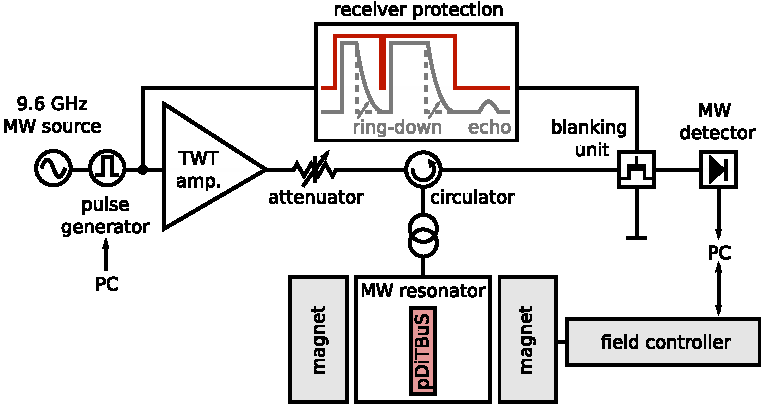
\includegraphics[width=1\textwidth]{./pulse/figures/pEPR_spectrometer_diagram.pdf}
	\caption{Diagram of a pulsed EPR spectrometer.}
	\label{fig:pepr_spectrometer_diagram}
\end{figure}

\subsection{Pulse Sequences and Measurement Techniques}
\subsubsection{The Refocused Spin Echo Sequence}
The Hahn Echo sequence consists of two pulses, the $\pi/2$ pulse and the $\pi$ pulse, separated in time by $\tau$: $\pi/2 - \tau - \pi - \tau - echo$. Initially, the macroscopic magnetization of the spin system is aligned along $\vec{B_0}$: $\vec{M}_0=M_Z~\vec{e_Z}$. The $\pi/2$ microwave pulse has such length $t_{\pi/2}$ and amplitude $B_1$ that, during the pulse, $\vec{M}$ nutates to the $xy$ plane, where it keeps precessing about $\vec{e_Z}$ after the end of the pulse. The difference in local environments for each individual spins in the spin packet, as well as the interactions between the spins, that make up $\vec{M}$, leads to slightly different precession frequencies $\omega_L^i$ of the spins. After some time $\tau$, the difference in the precession frequencies translates into the differences in phases so that the vector sum of the excited spins averages down to $\vec{0}$ for sufficiently long $\tau$. In other words, the excited spin packet dephases with time. The dephasing due to different local spin environments can be reversible if the deviations of the precession frequencies do not depend on time, as is the case for separated electrons in an inhomogeneous solid. In such case, a $\pi$ pulse can be applied to the spin system to flip every single spin in the dephased spin packet by 180$\deg$ in a plane containing $\vec{e}_Z$, so that the spins keep precessing in the $xy$ plane, but the direction of precession is inverted for them, leading to the effect that is opposite to the initial dephasing. So a $\tau$ after the $\pi$ pulse excites the spin packet, the accumulated phase differences become the smallest and the packet recovers its macroscopic magnetization $\vec{M}$ that oscillates in the $xy$ plane with $\langle\omega_L^i\rangle$ and can be detected. The recovered $\vec{M}$ at $t=\tau$ after the $\pi$ pulse is called the refocused spin echo. The difference in $\omega_L^i$ leads to a further dephasing of the considered spin packet and to the vanishing of $\vec{M}$.\\
\subsubsection{Spin Echo Decay and Phase Memory Time}


\subsubsection{Inversion Recovery and Spin-Lattice Relaxation Time}

\subsection{Broad-Band Excitation and Instantaneous Diffusion}
In Section /// it is shown that in a densely packed radical system, as in a TEMPO-Salen cathode film, the phase memory time can be shorter than $T_m\leq100$~ns. That is, the spin echo is decaying by $e\approx3$ times at $t=100$~ns. The short phase memory time limits the duration of the pulse sequence at which the echo is detectable. For a $\pi/2-\tau-\pi-\tau-echo$ sequence, with a hardware limitation on $\tau\geq t_d\approx100$~ns, the shorter pulse sequence becomes longer than $t>200$~ns. By this time, the spin echo decreases by $e^2\approx7$ times and may be comparable to noise. The limitations imposed by the finite $T_m$ and $t_d$ force one to use shorter microwave pulses. 
\par
A short microwave pulse may have a spectral width comparable to the width of the observed spectrum. According to the Fourier theorem, the spectral width of a pulse is inversely proportional to the pulse length: $\Delta\omega\sim 1/t_p$. A spectrum of a 100~ns long rectangular pulse shown in Figure /// is ///MHz wide (FWHM). 

\begin{figure}[h]
\center
	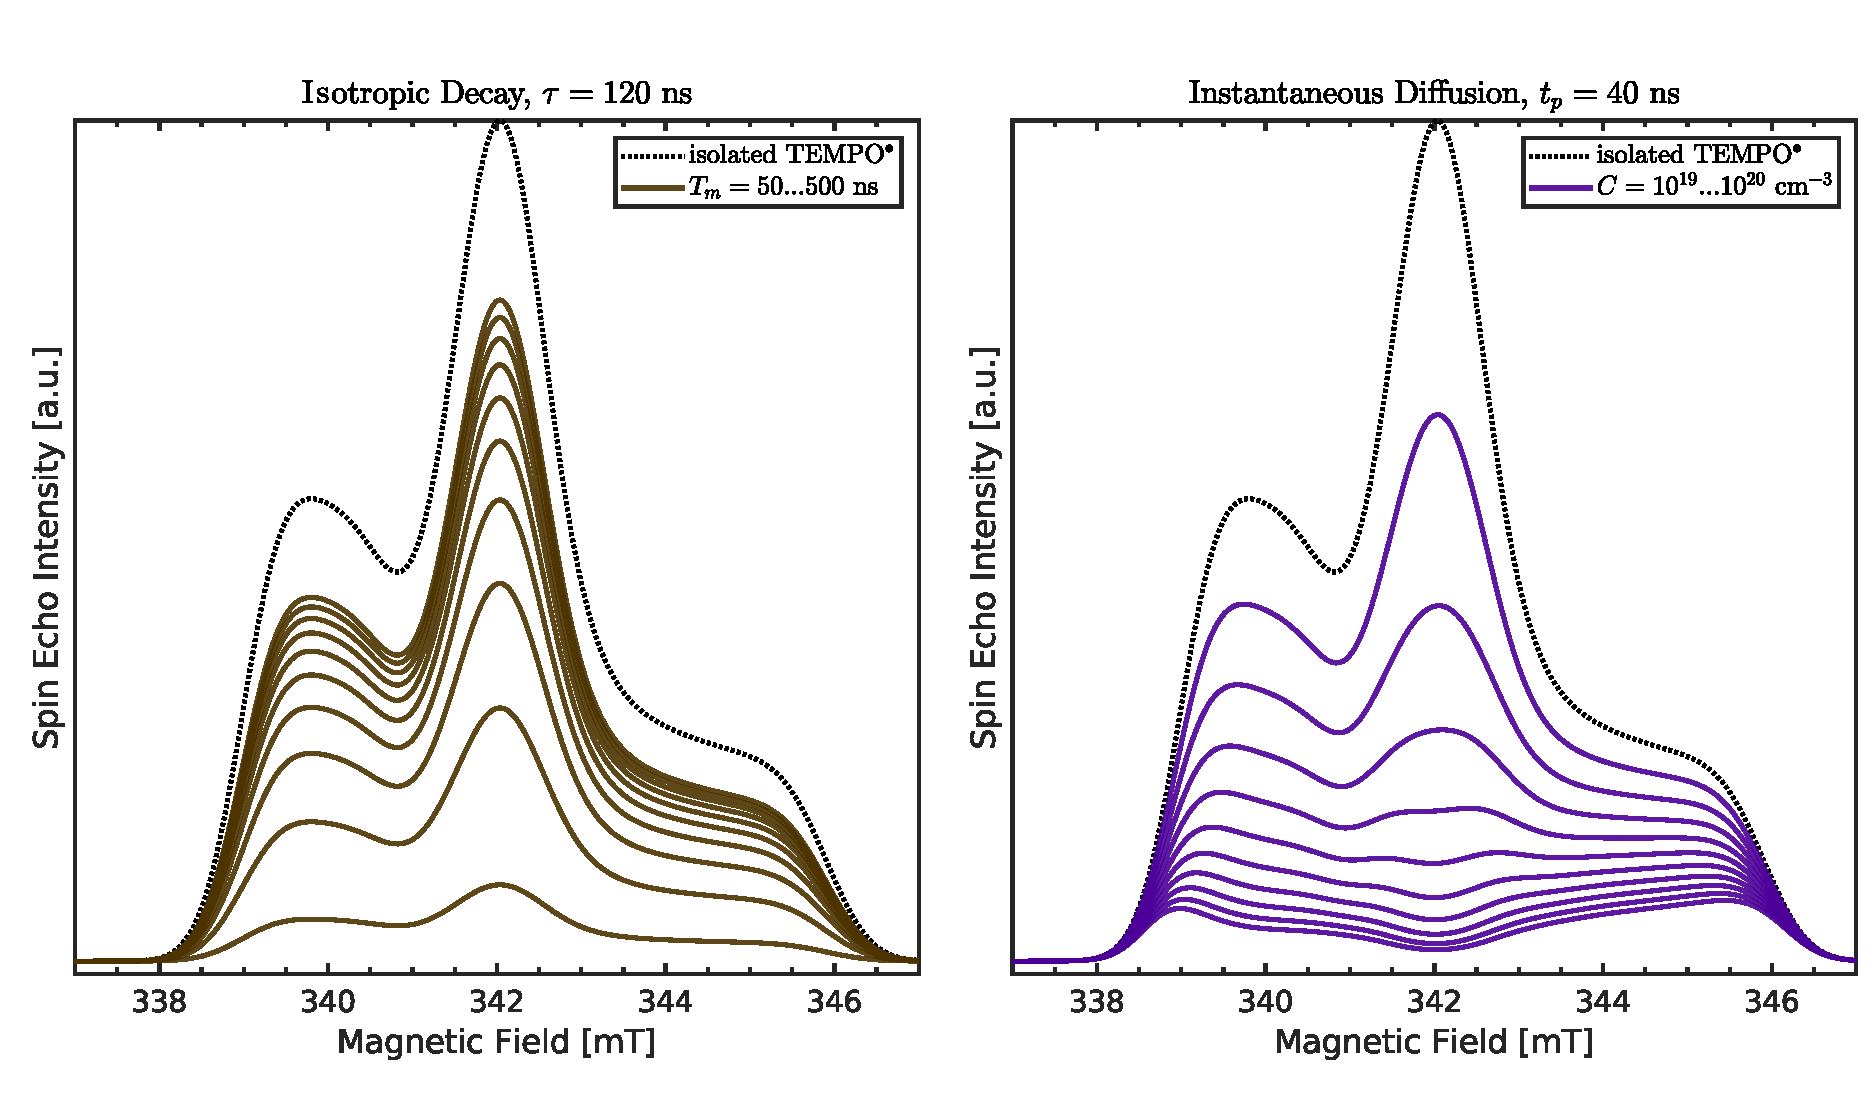
\includegraphics[width=1\textwidth]{./pulse/figures/FGMR/ID/ID_vs_ISO.pdf}
	\caption{Distortions of a nitroxide FSE spectrum caused by isotropic spin relaxation (left) and instantaneous diffusion (right).}
	\label{fig:iso_vs_id}
\end{figure}


\section{Pulsed EPR Spectroscopy of a charged pDiTBuS Cathode film}


\begin{figure}[h]
\center
	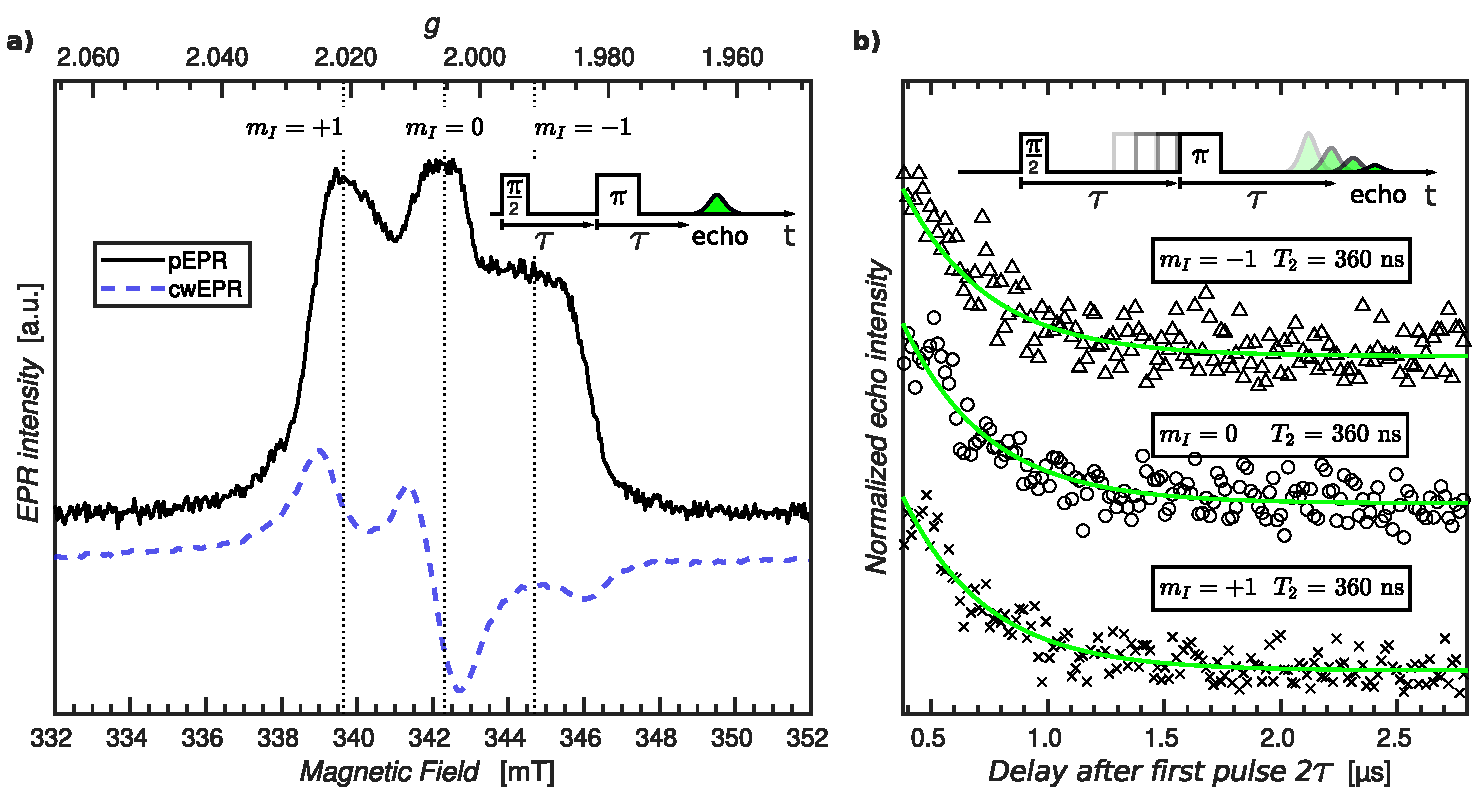
\includegraphics[width=1\textwidth]{./pulse/figures/SAW_Figure_8.pdf}
	\caption{X}
	\label{fig:FSE_vs_CW_DiTS_rel_times}
\end{figure}

\begin{figure}[h]
\center
	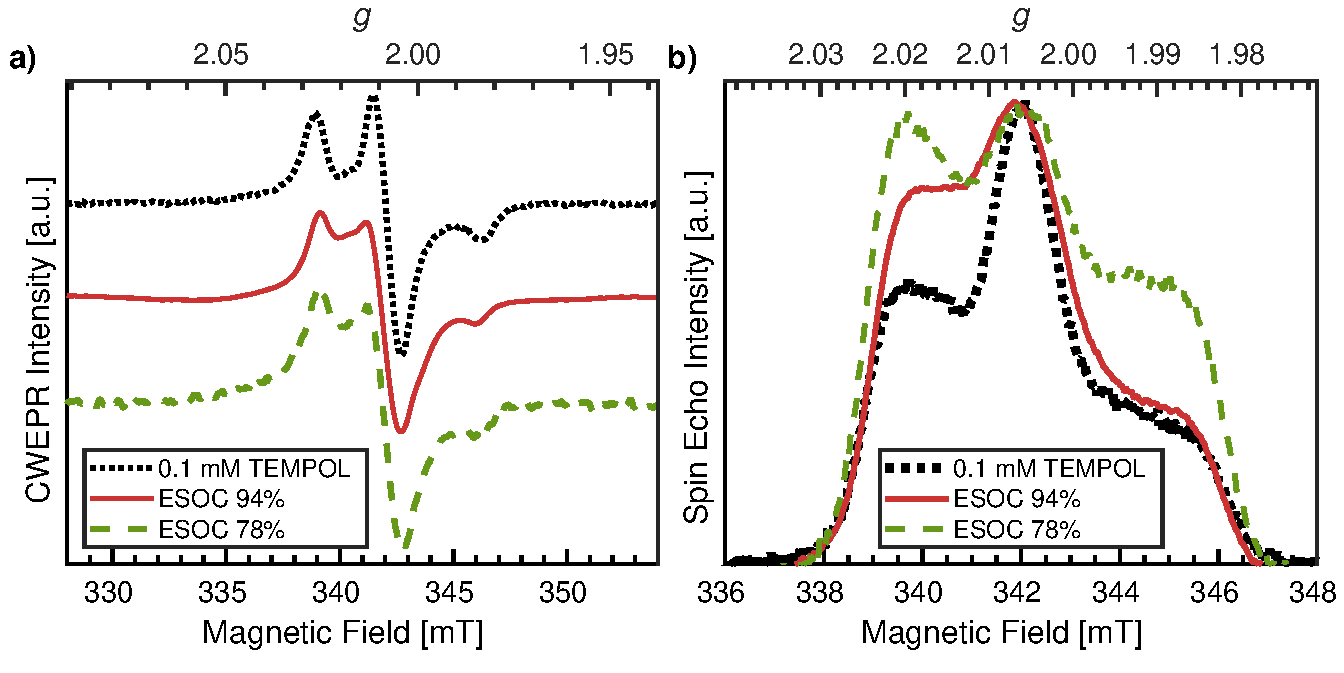
\includegraphics[width=1\textwidth]{./pulse/figures/Figure_3.pdf}
	\caption{X}
	\label{fig:FSE_vs_CW_DiTBuS}
\end{figure}

\begin{figure}[h]
\center
	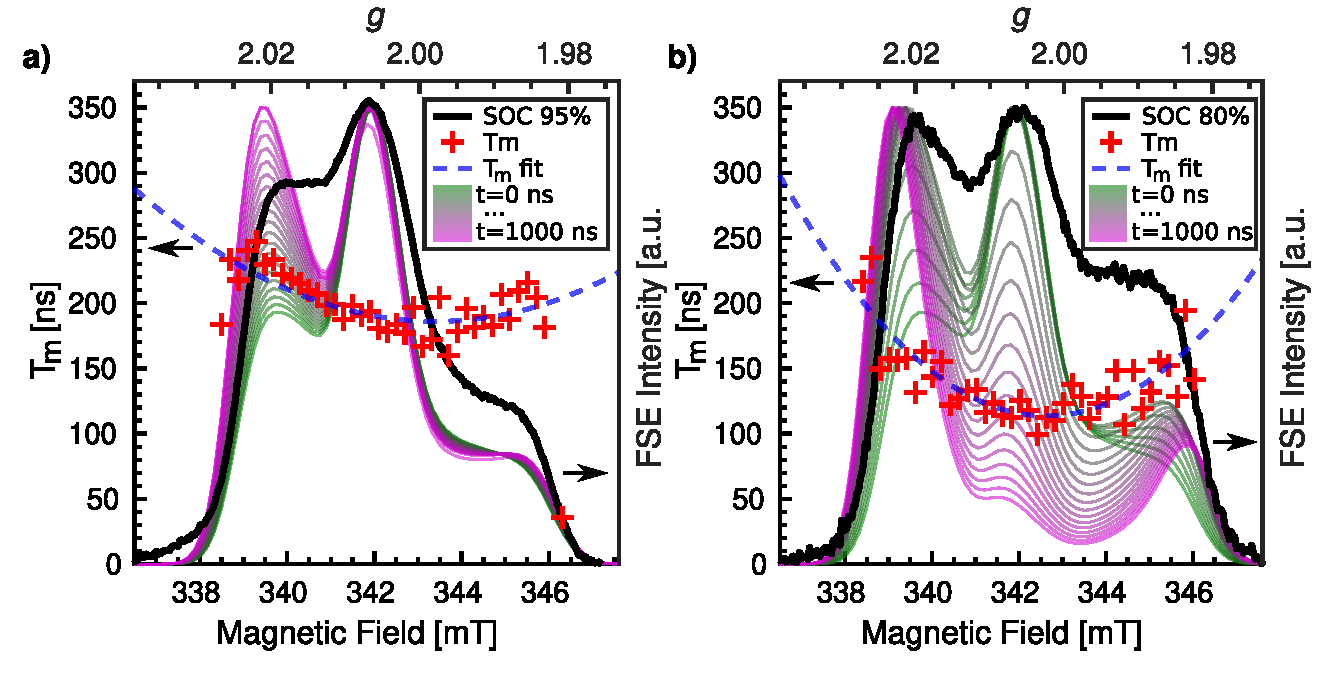
\includegraphics[width=1\textwidth]{./pulse/figures/Figure_6_maintext_col_MOD.pdf}
	\caption{X}
	\label{fig:FSE_reconstruction_with_T2}
\end{figure}


\begin{figure}[h]
\center
	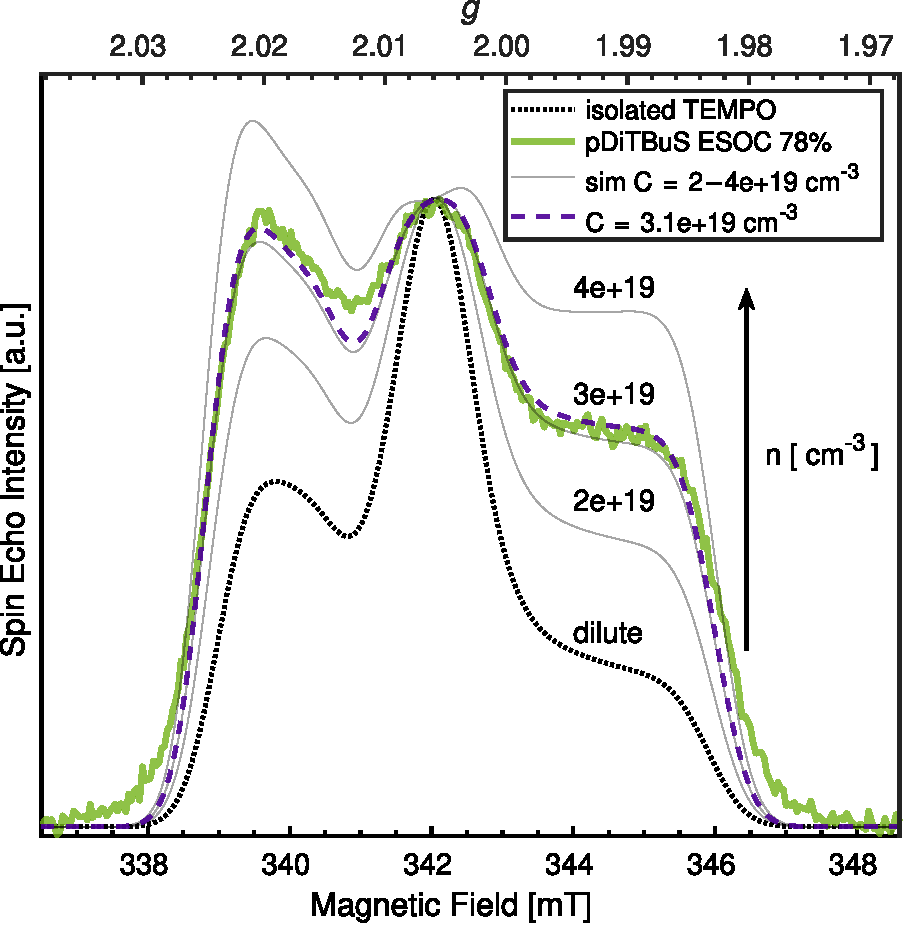
\includegraphics[width=0.45\textwidth]{./pulse/figures/Figure_4.pdf}
	\caption{X}
	\label{fig:FSE_with_ID_DiTBuS}
\end{figure}



\subsection{Field Swept Echo of a charged pDiTBuS Cathode film}
\begin{figure}[h]
\center
	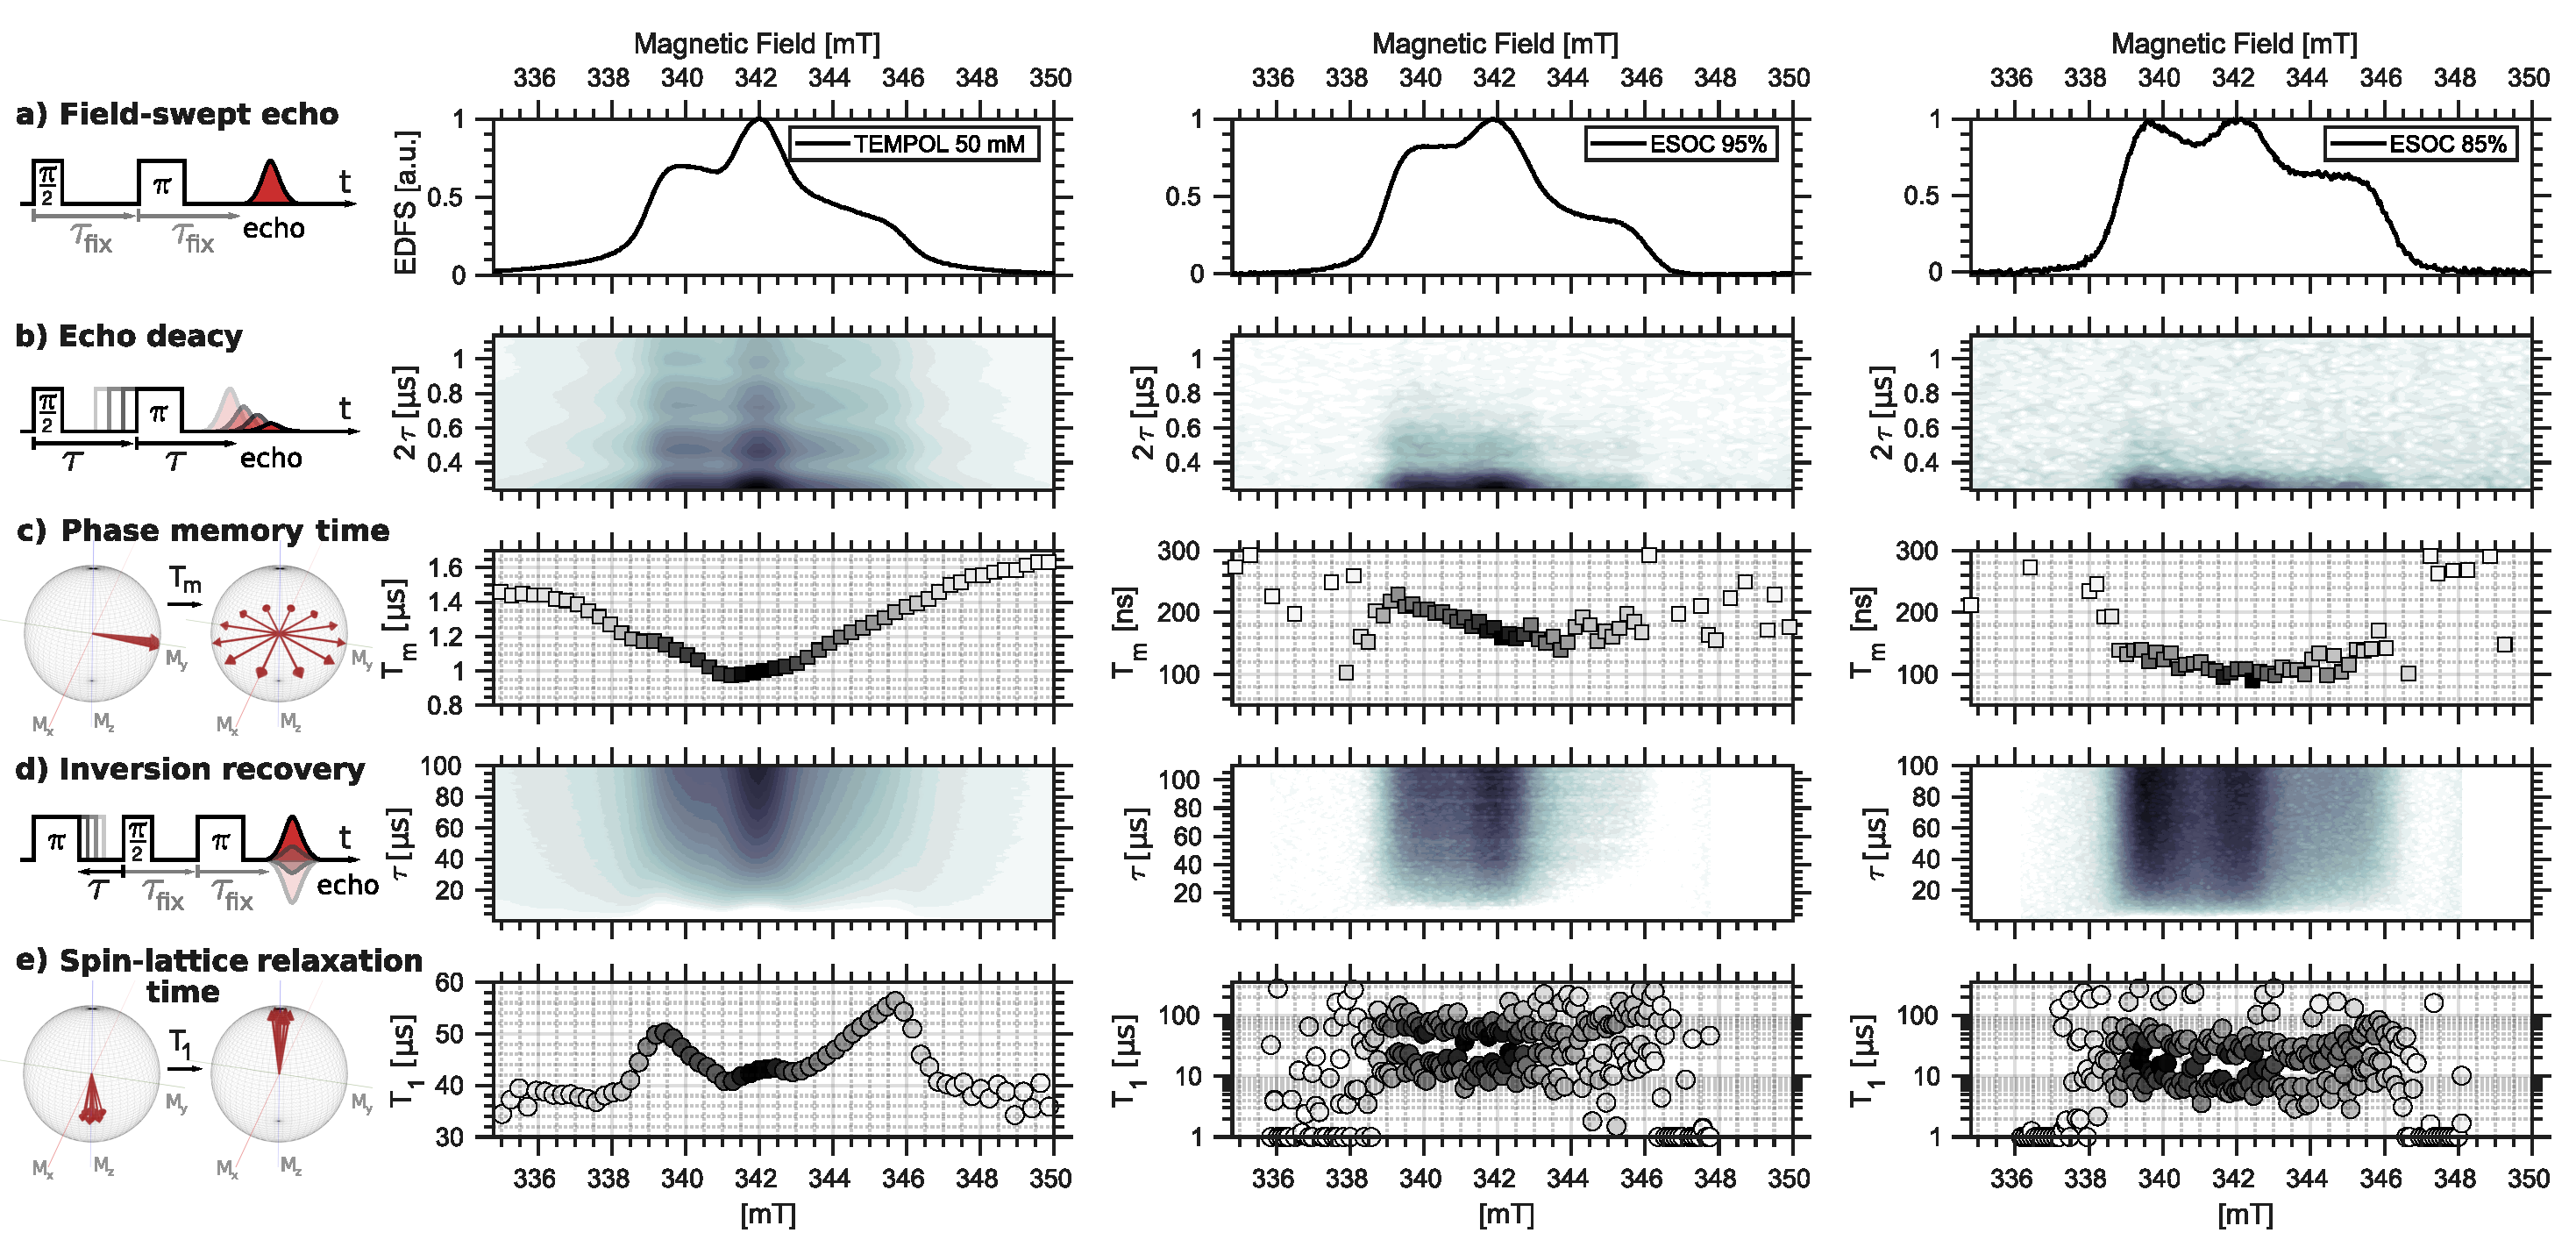
\includegraphics[width=1\textwidth]{./pulse/figures/FSE_DTBS_FSE_RELAX_T1Tm.pdf}
	\caption{XXX}
	\label{fig:Figure_FSE2}
\end{figure}


\subsection{Estimation of Local Spin Concentrations with Instantaneous Diffusion}
\subsection{Spin Relaxation in a charged pDiTBuS Cathode Film}

\section{Pad{\'e}-Laplace Deconvolution of Polyexponential Decay Signals}
\label{sec:pade-laplace}
The echo decay and inversion recovery transients measured in the corresponding experiments may contain multiple exponential decay components. The conventional method of determining the distribution of the decay components in a transient decay is the Laplace inversion, where the signal in the time domain $s(t)$ is converted into its Laplace image $L(p)=\int\limits_{0}^{+\infty}s(t)e^{-pt}\mathrm{d}t$ in the time-constant domain $p=1/t$, where the peaks of $L(p)$ give the decay constants that make up the signal. However, for the noisy signal, the direct calculation of the Laplace transform brings in artifacts that drastically vary with the noise. The signal-to-noise ratio (SNR) of the recorded data makes it difficult to apply the Laplace inversion to determine the number of the decay components, as the Laplace transform is unstable at that SNR. \\ 


The Pad{\'e}-Laplace method comes useful for analyzing noisy polyexponential decays as it was demonstrated in Ref.~\cite{Hellen_2005}. The idea of the Pad{\'e}-Laplace method is to analyze the Pad{\'e} approximation of the Taylor expansion of the $L(p)$ in the vicinity of one of the expected decay constants $p_0$, rather than considering the $L(p)$ fully. This way of signal decomposition is stable against the noise for SNR$<$10 (see Figure~\ref{fig:Figure_S7}). The number of exponents detected by the Pad{\'e}-Laplace method as well as their locations in the $p$ space may vary depending on the expansion point $p_0$. We considered $p_0=1/t_{1/2}$ where $t_{1/2}$ is the time at which the signal amplitude halves.\\

We implemented the following algorithm to detect the number of exponents in the decaying transient $s(t)$:\\

First, a point $p_0=1/t_{1/2}$ was chosen, at which $s(t)$ halves.\\

Then, 11 coefficients of the Taylor expansion of the Laplace transform $L(p)$ were calculated in the vicinity of $p \rightarrow p_0$\\

\begin{equation}
L(p)\vert_{p \rightarrow p_0} = \sum_{n=0}^{11} d_i (p-p_0)^i
\end{equation}
with
\begin{equation}
d_i = \frac{1}{i!}\left(\frac{d^{(i)}L}{dp^{(i)}}\right)_{p=p0}
\end{equation}
where the derivatives $\frac{d^{(i)}L}{dp^{(i)}}$ are computed numerically at the point $p=p_{0}$ from the discrete signal $s(t) = (t_j,f_j),~j=1~...~M$:
\begin{equation}
\frac{d^{(i)}L}{dp^{(i)}}= \sum_{j=2}^{M-1}(-t_j)^ie^{(-p_0t_j)}f_j + \frac{1}{2}\left((-t_1)^ie^{(-p_0t_1)}f_1+(-t_M)^ie^{(-p_0t_M)}f_M \right)
\end{equation}


Then the Taylor expansion for $L(p)$ was approximated in the vicinity of $p_0$ with the Pad{\'e} polynomials a(p) and b(p) of orders $n=5$ and $n=6$ respectively:\\

\begin{equation}
\label{eq:pade}
L(p)\vert_{p \rightarrow p_0} = d_0+d_1(p-p_0)+\dots+d_{11}(p-p_0)^{11}=\frac{a_0 + a_1(p-p_0) + \dots + a_5(p-p_0)^5}  {1 + b_1(p-p_0)+ \dots+ b_6(p-p_0)^6}
\end{equation}

The equation \ref{eq:pade} is multiplied by the the denominator and the prefactors at $(p-p_0)^{n}$ for $n=6\dots11$ are compared. This defines a system of linear equations on coefficients $b_i$:\\


\begin{equation}\label{eq:matrix}
  \begin{pmatrix}
    d_{5} & d_{4} & d_{3} & d_2 & d_1 & d_0\\
    d_6 & d_5 & d_4 & d_3 & d_2 & d_1\\
    d_7 & d_6 & d_5 & d_4 & d_3 & d_2\\
    d_8 & d_7 & d_6 & d_5 & d_4 & d_3\\
    d_9 & d_8 & d_7 & d_6 & d_5 & d_4\\
    d_{10} & d_9 & d_8 & d_7 & d_6 & d_5
  \end{pmatrix}
       \begin{pmatrix}
   b_1\\
   b_2\\
   b_3\\
   b_4\\
   b_5\\
   b_6
   \end{pmatrix}
  =
    \begin{pmatrix}
   -d_6\\
   -d_7\\
   -d_8\\
   -d_9\\
   -d_{10}\\
   -d_{11}
   \end{pmatrix}
\end{equation}

From \ref{eq:matrix}, $b_i$ are found. The coefficients $a_i$ are found from ${d}$ and ${b}$.\\

Finally, the Pad{\'e} approximation $P=\frac{a}{b}$ is constructed and its poles are analyzed. The position of the poles reveal the decay constants. The residues at the poles may give the amplitudes of the decay components, but this was not used in the present study.

\begin{figure}[ht!]
\center
	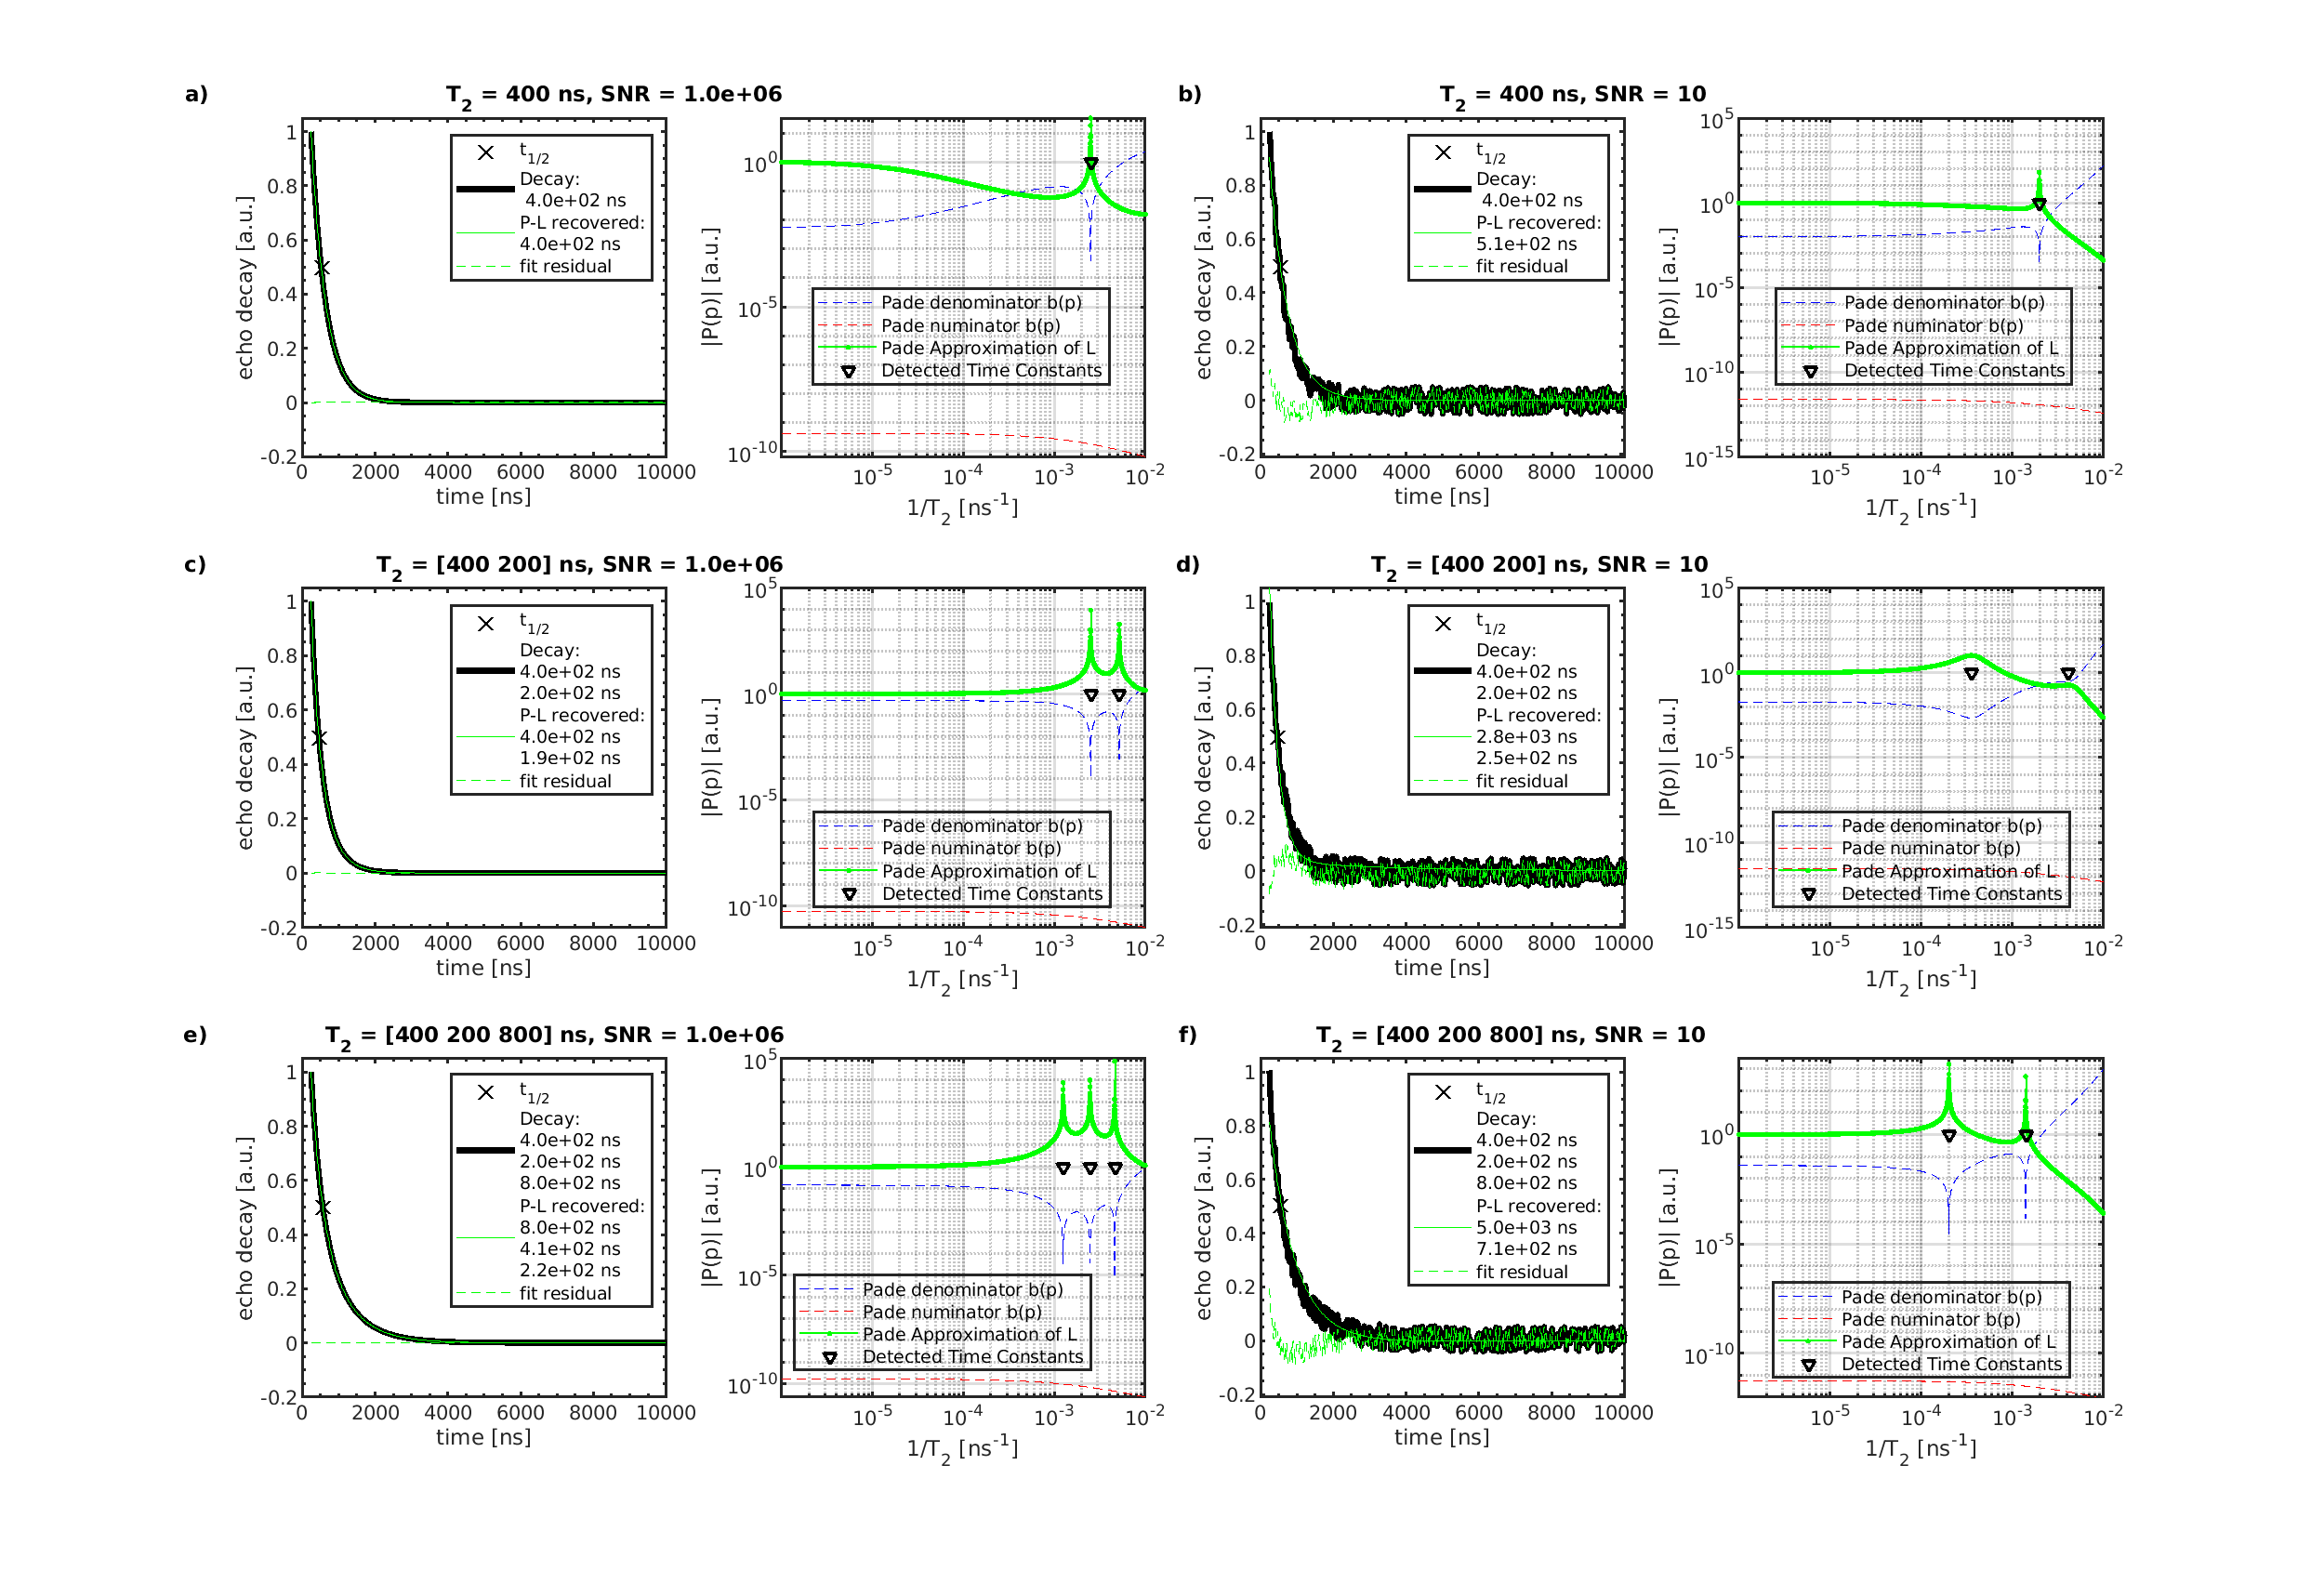
\includegraphics[width=1\textwidth]{./pulse/figures/Figure_S7.pdf}
	\caption{Pad{\'e}-Laplace deconvolution of the mock data containing two decay constants with various signal-to-noise (SNR) ratios.}
	\label{fig:Figure_S7}
\end{figure}


\newpage
\subsection{Pad{\'e}-Laplace Deconvolution of the Echo-Decay and Inversion-Recovery Transients}
\label{pade_laplace_T2}
We used the Pad{\'e}-Laplace method to determine the number of the decay constants in the signals and used multiexponential fits to adjust the decay constants and their amplitudes. For the echo decay transients the best fits were monoexponential fits, even though the Pade-Laplace analysis initially showed biexponential behavior for pDiTBuS with major contribution from the fast decay constants in the order of the detector's dead time. All recorded echo decay transients contain oscillations due to the ESEEM effect. The oscillations were excluded from the analysis as shown in the 'fit area' on the plots in Figure~\ref{fig:Figure_S9}, Figure~\ref{fig:Figure_S11} and Figure~\ref{fig:Figure_S13}.

\newpage
\subsubsection{Echo Decay in 50 mM TEMPOL}
\begin{figure}[ht!]
\center
	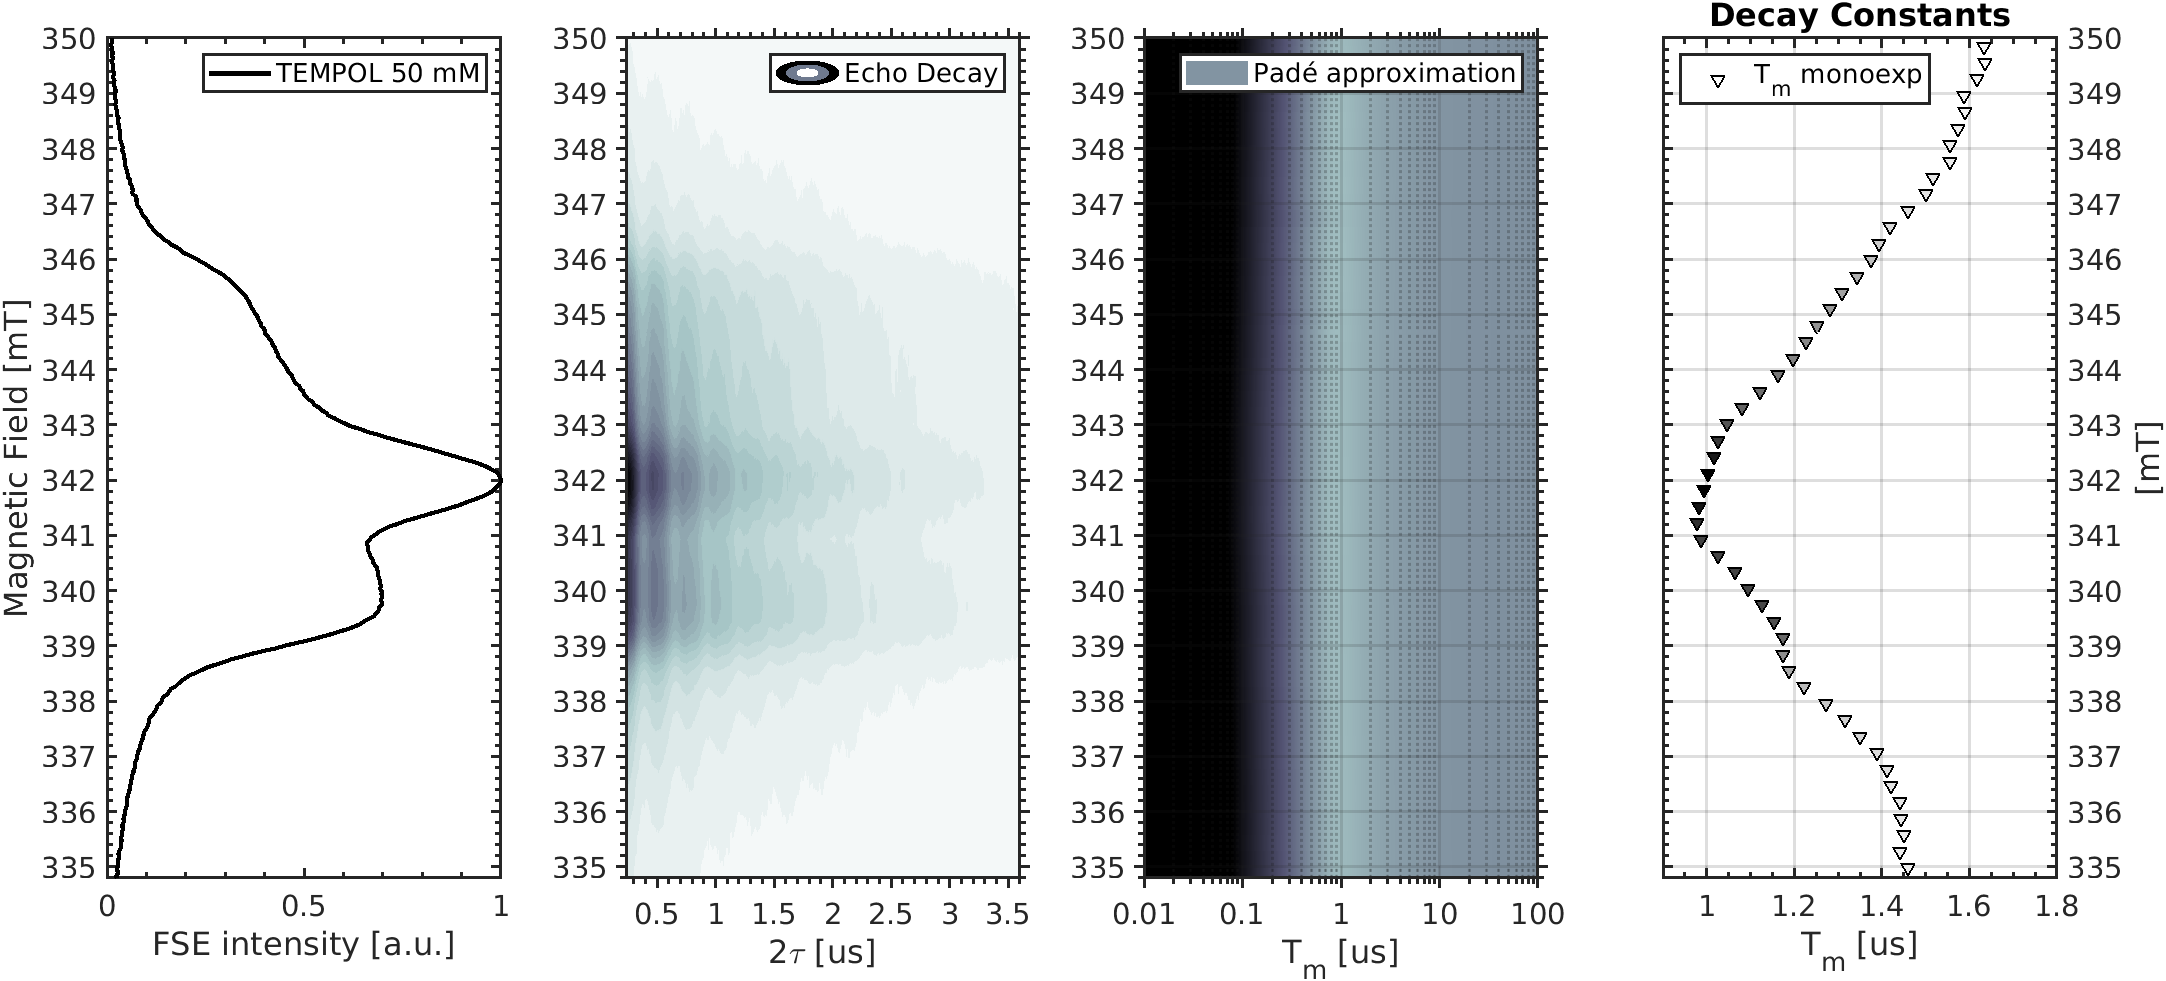
\includegraphics[width=1\textwidth]{./pulse/figures/Figure_S8.png}
	\caption{Pad{\'e}-Laplace deconvolution of the field-swept spin echo decay in a frozen 50~\si{\milli\Molar}  solution of TEMPOL in Dichloromethane:Acetonitrile glass (3:1). One decay component detected with Pade-Laplace (triangles, right panel). Monoexponential fit (squares for faster component, circles for slower component, right panel). Temperature 5K.}
	\label{fig:Figure_S8}
\end{figure}

\begin{figure}[ht!]
\center
	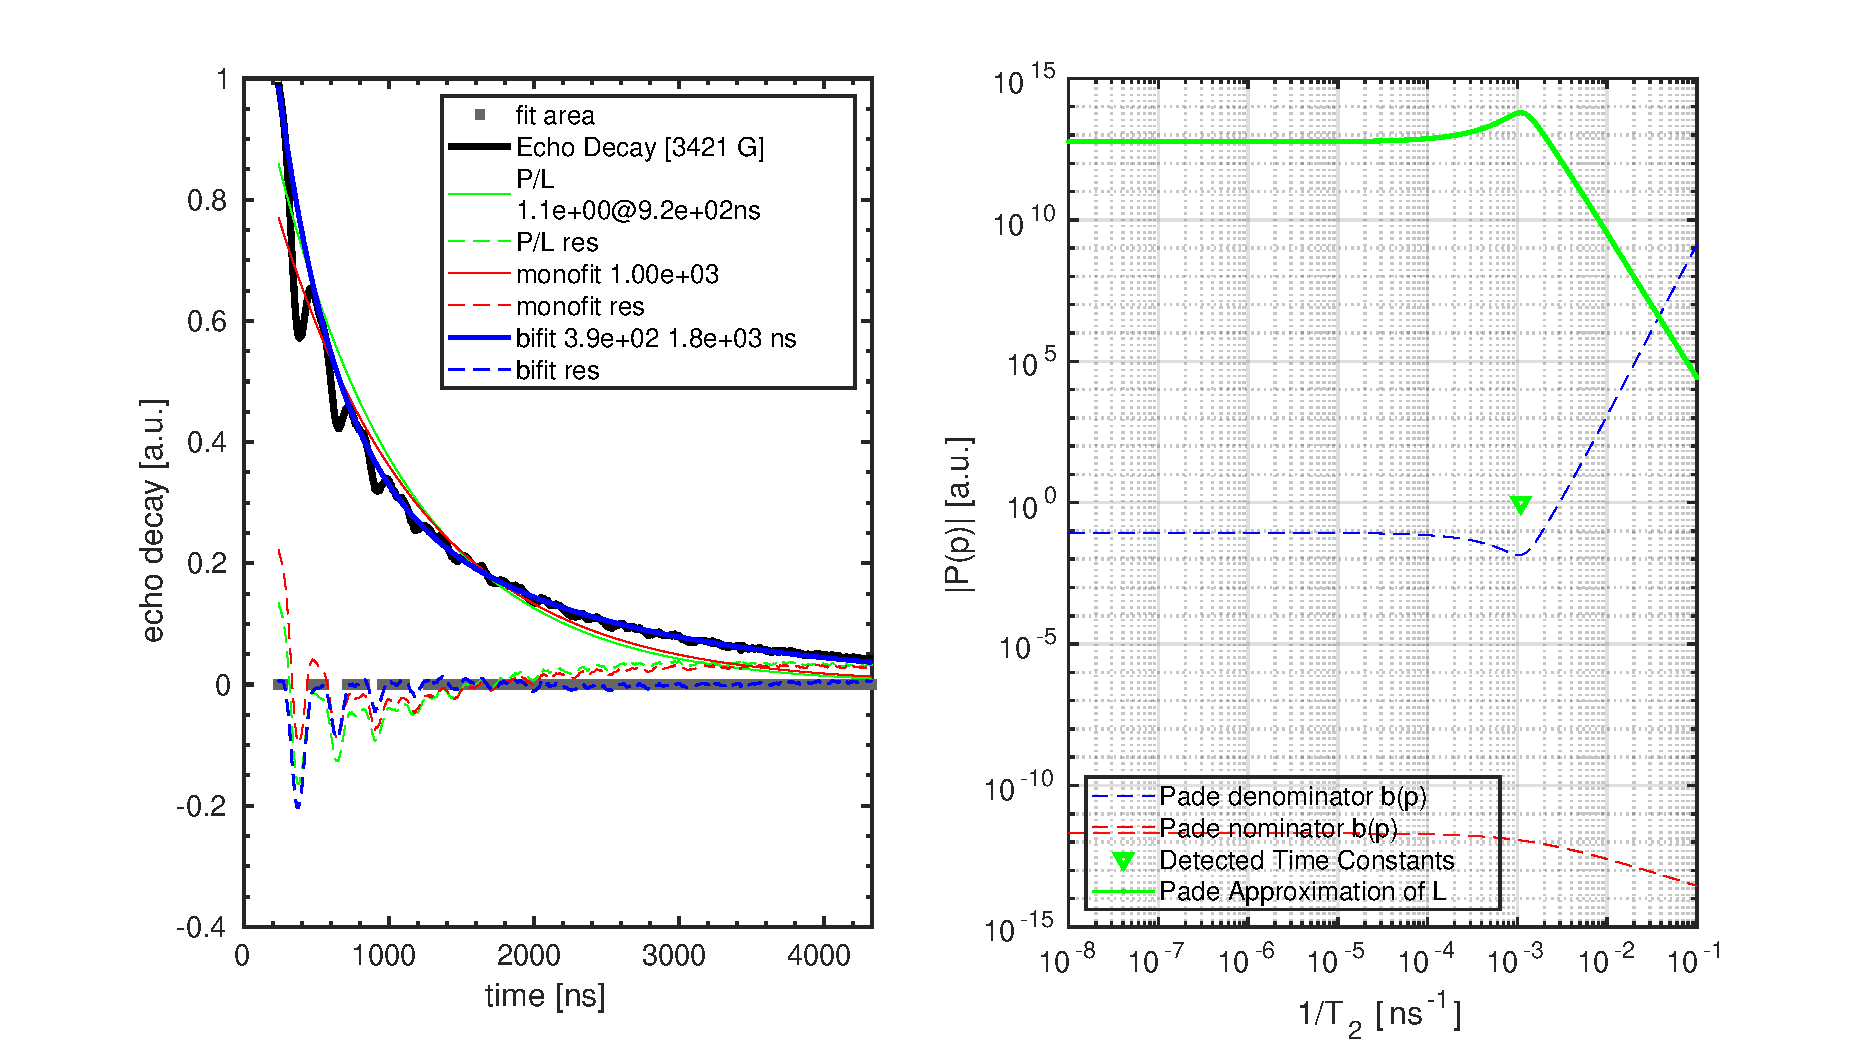
\includegraphics[width=0.9\textwidth]{./pulse/figures/Figure_S9.pdf}
	\caption{Fits of the echo decay transient in the frozen 50~\si{\milli\Molar}  TEMPOL solution at the central spectral peak ($m_I=0$, 342~mT). Pad{\'e}-Laplace deconvolution the transient vs. free monoexponential fit vs biexponential fit. Temperature 5K. Data was fit in the 'fit area' region. ESEEM oscillations were excluded from the data for fit and Pade-Laplace analysis.}
	\label{fig:Figure_S9}
\end{figure}


\newpage
\subsubsection{Echo Decay in DiTBuS 95\% ESOC}
\begin{figure}[h]
\center
	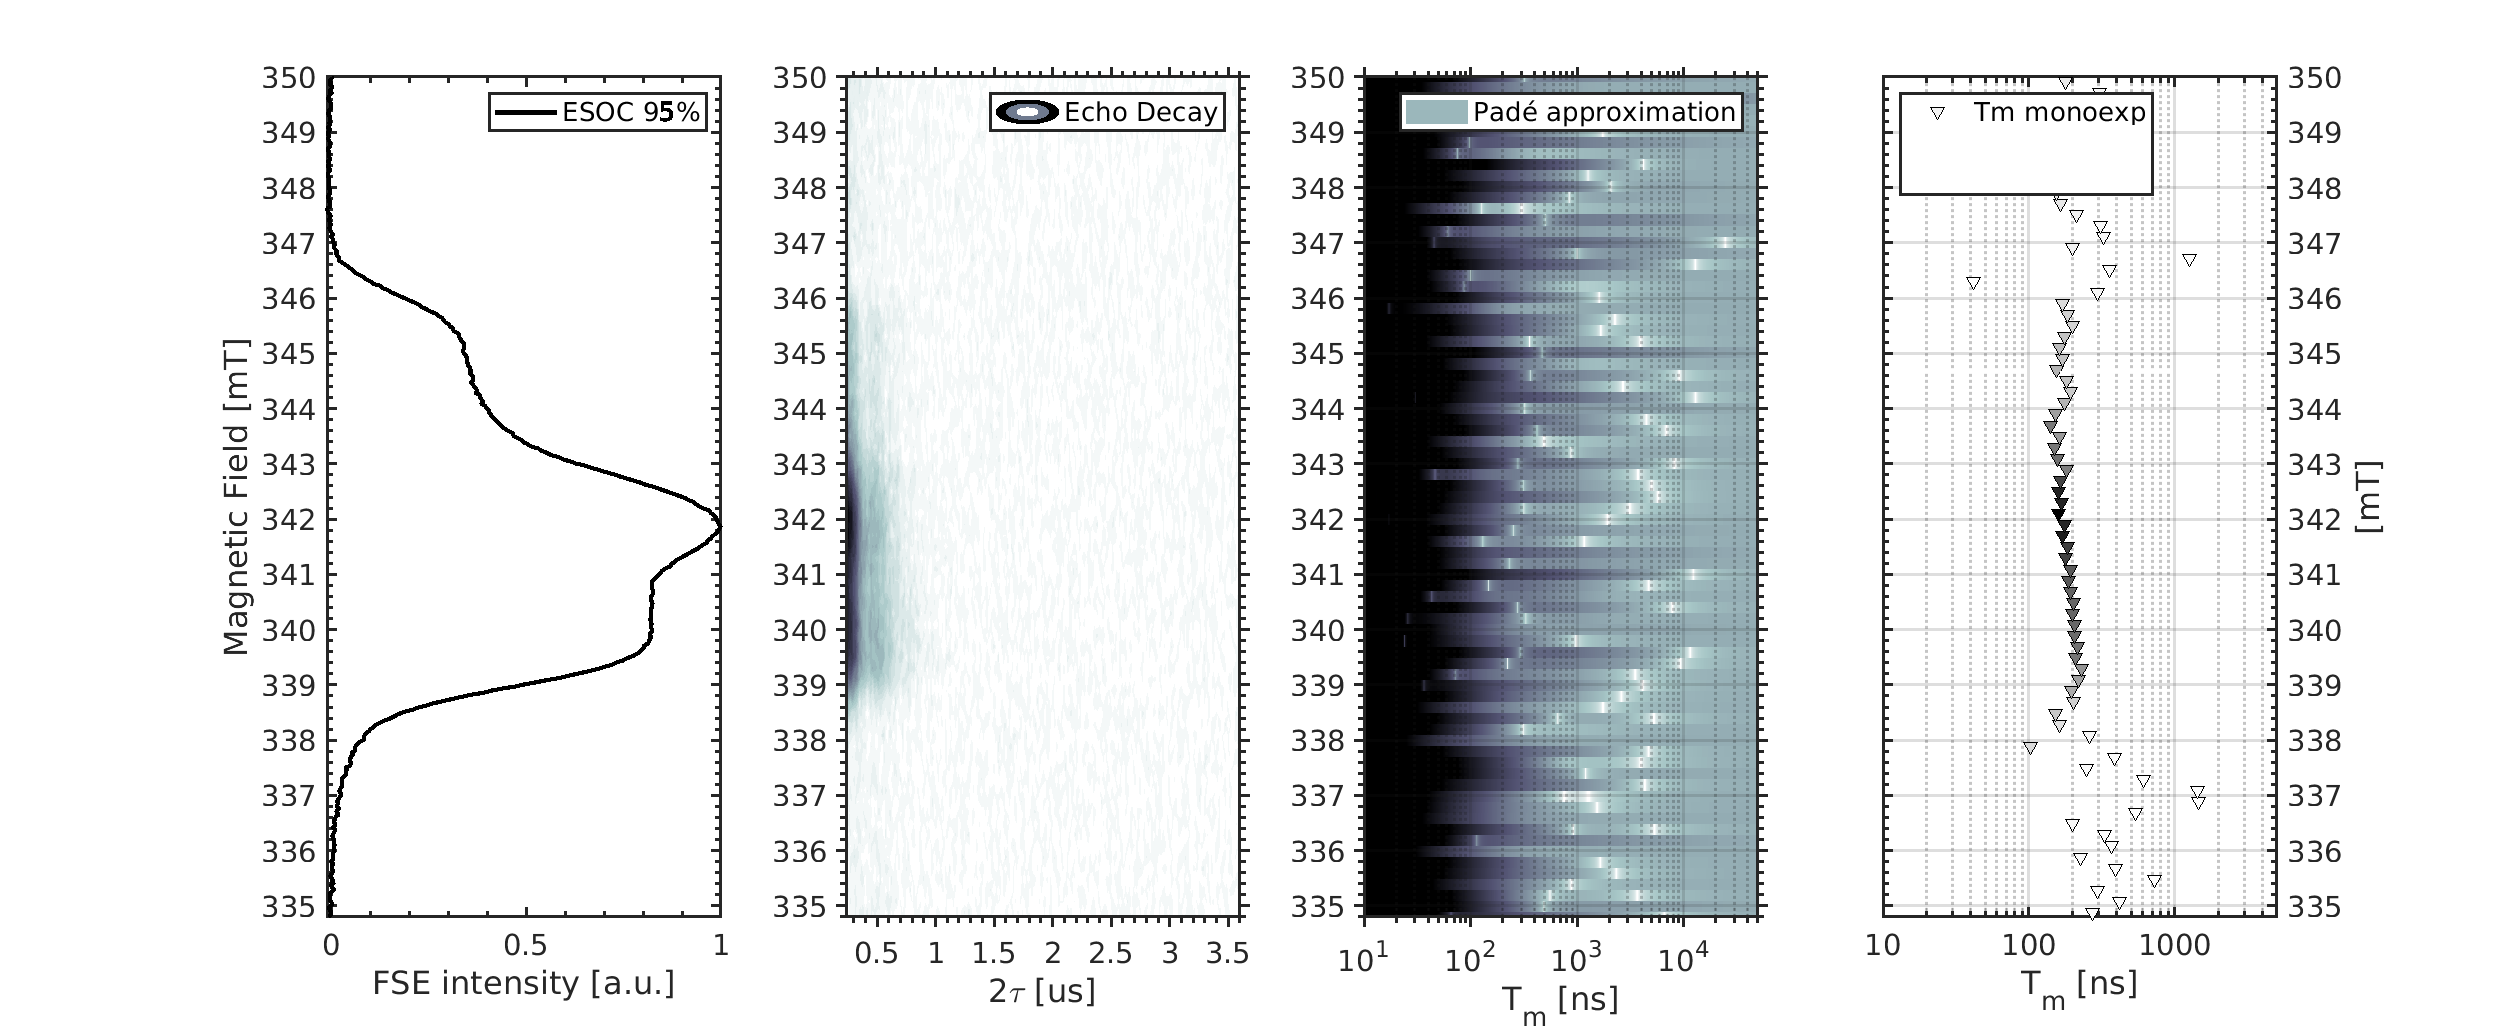
\includegraphics[width=1\textwidth]{./pulse/figures/Figure_S10.pdf}
	\caption{Pad{\'e}-Laplace deconvolution of the field-swept spin echo decay in the pDiTBuS film at 95\%~ESOC. Temperature 5K.}
	\label{fig:Figure_S10}
\end{figure}


\begin{figure}[ht!]
\center
	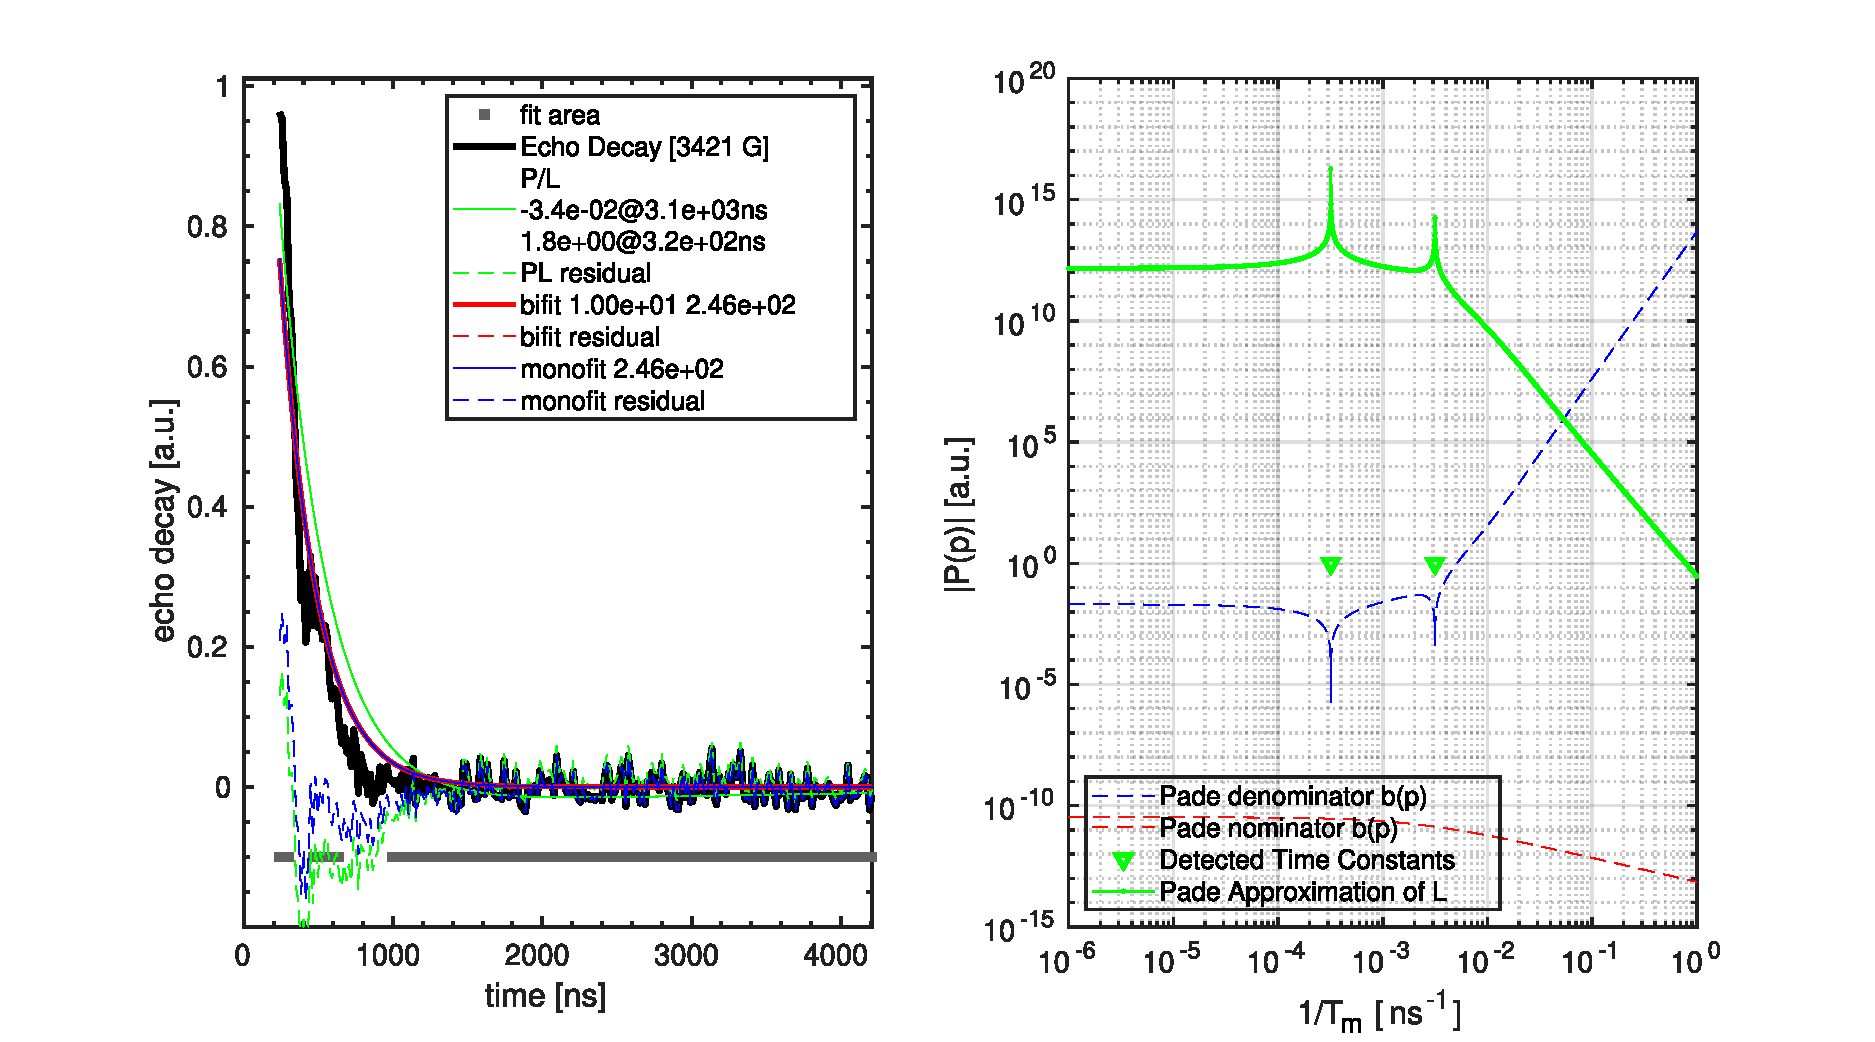
\includegraphics[width=0.9\textwidth]{./pulse/figures/Figure_S11.pdf}
	\caption{Fits of the echo decay transient in the pDiTBuS film at 95\%~SoC at the central spectral peak ($m_I=0$, 342~mT). Pad{\'e}-Laplace deconvolution the transient vs. free monoexponential fit vs biexponential fit. Temperature 5K. Data was fit in the 'fit area' region. ESEEM oscillations were excluded from the data for fit and Pade-Laplace analysis.}
	\label{fig:Figure_S11}
\end{figure}


\newpage
\subsubsection{Echo Decay in DiTBuS 85\% ESOC}

\begin{figure}[h]
\center
	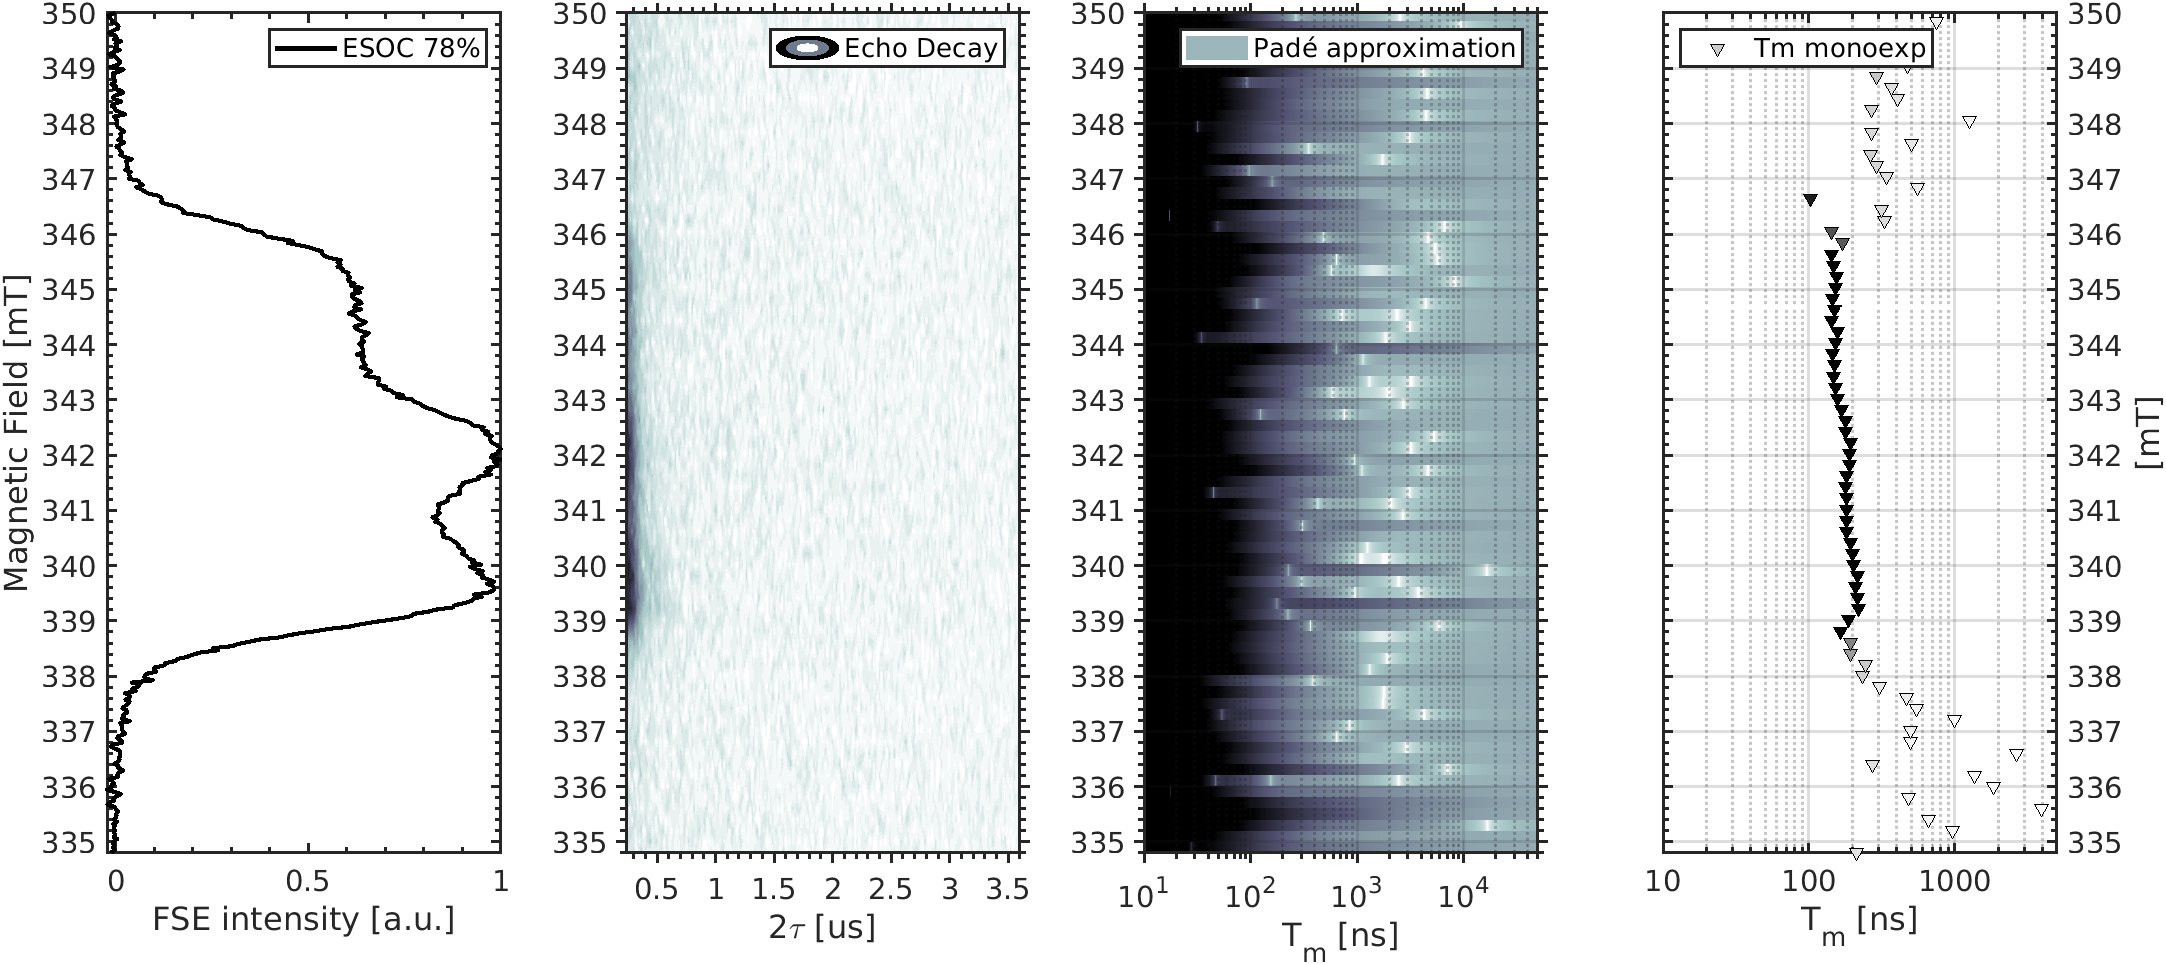
\includegraphics[width=1\textwidth]{./pulse/figures/Figure_S12.png}
	\caption{Pad{\'e}-Laplace deconvolution of the field-swept spin echo decay in a pDiTBuS film at 85\%~ESOC. Temperature 5K.}
	\label{fig:Figure_S12}
\end{figure}

\begin{figure}[ht!]
\center
	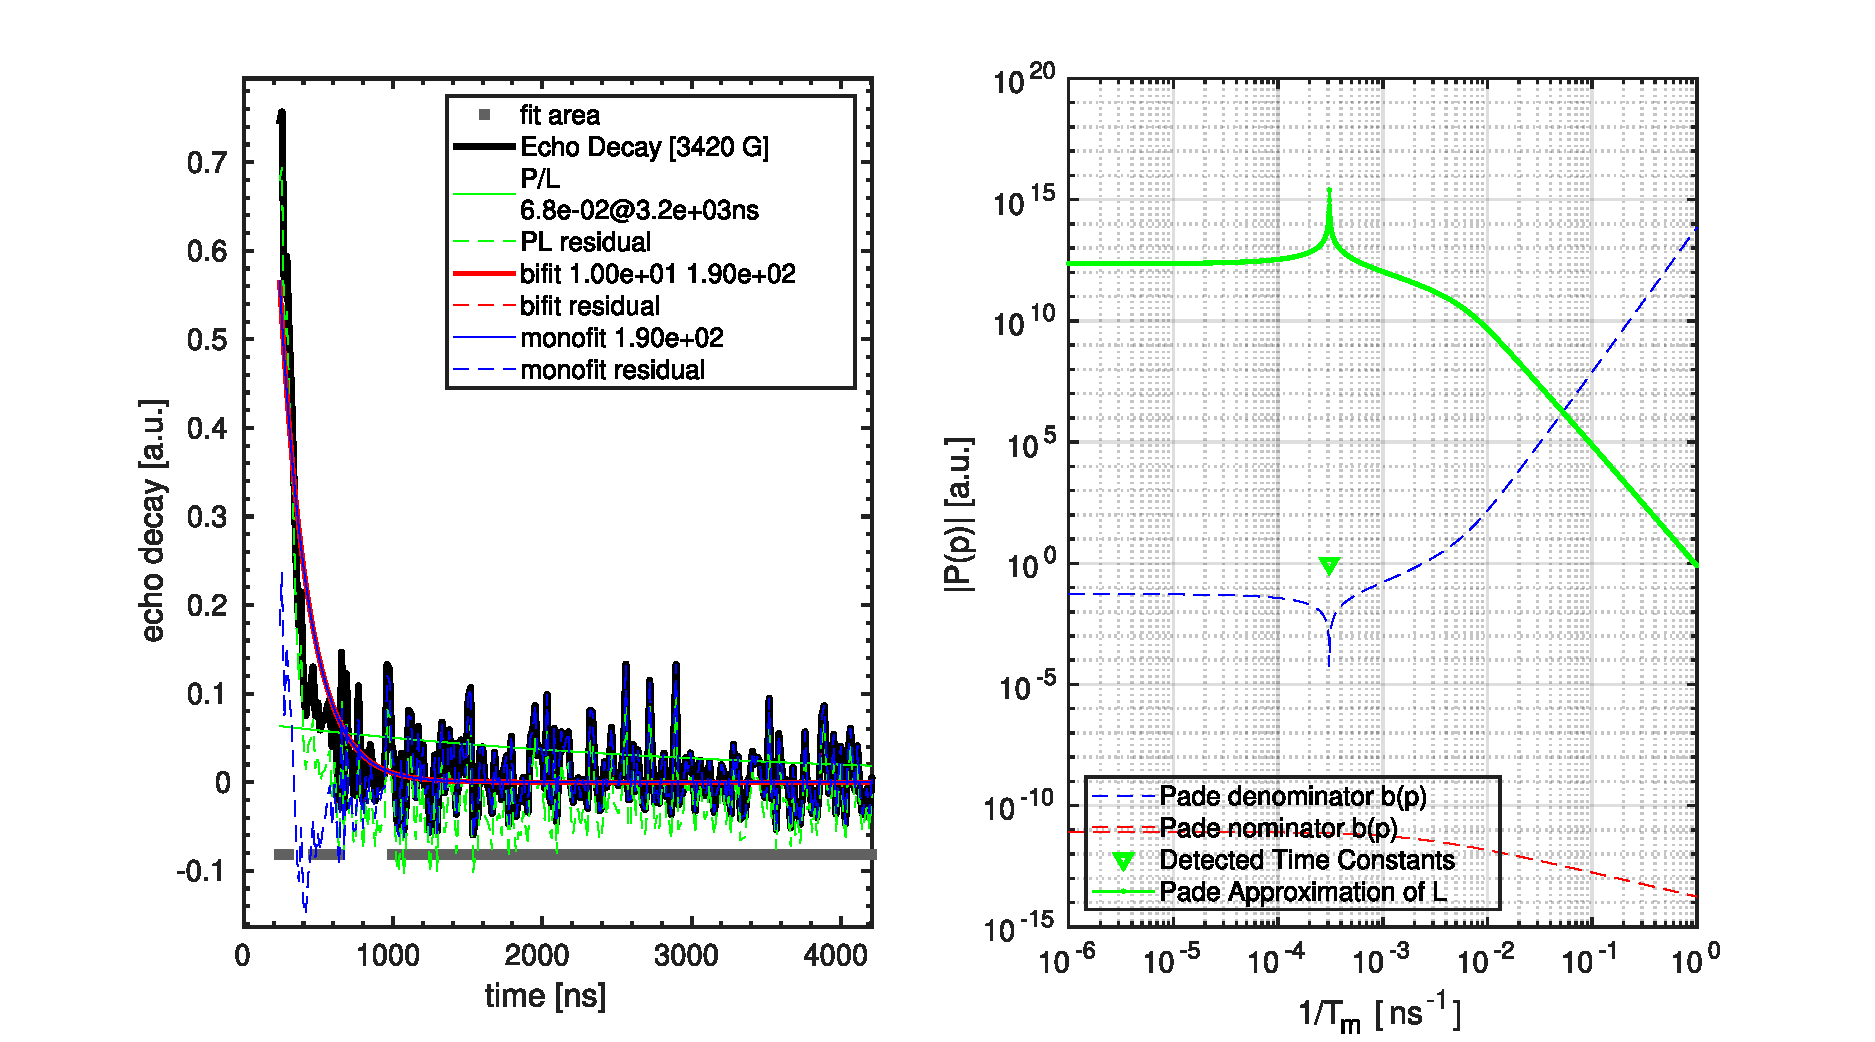
\includegraphics[width=0.9\textwidth]{./pulse/figures/Figure_S13.pdf}
	\caption{Pad{\'e}-Laplace deconvolution, biexponential and monoexponential fits of the spin echo decay in a pDiTBuS film at 85\%~SoC at the $m_I=0$ spectral position. Temperature 5K. Data was fit in the 'fit area' region. ESEEM oscillations were excluded from the data for fit and Pade-Laplace analysis.}
	\label{fig:Figure_S13}
\end{figure}



\newpage
\subsubsection{Inversion Recovery in 50 mM TEMPOL}
\label{esi:pade_laplace_T1}
\begin{figure}[h]
\center
	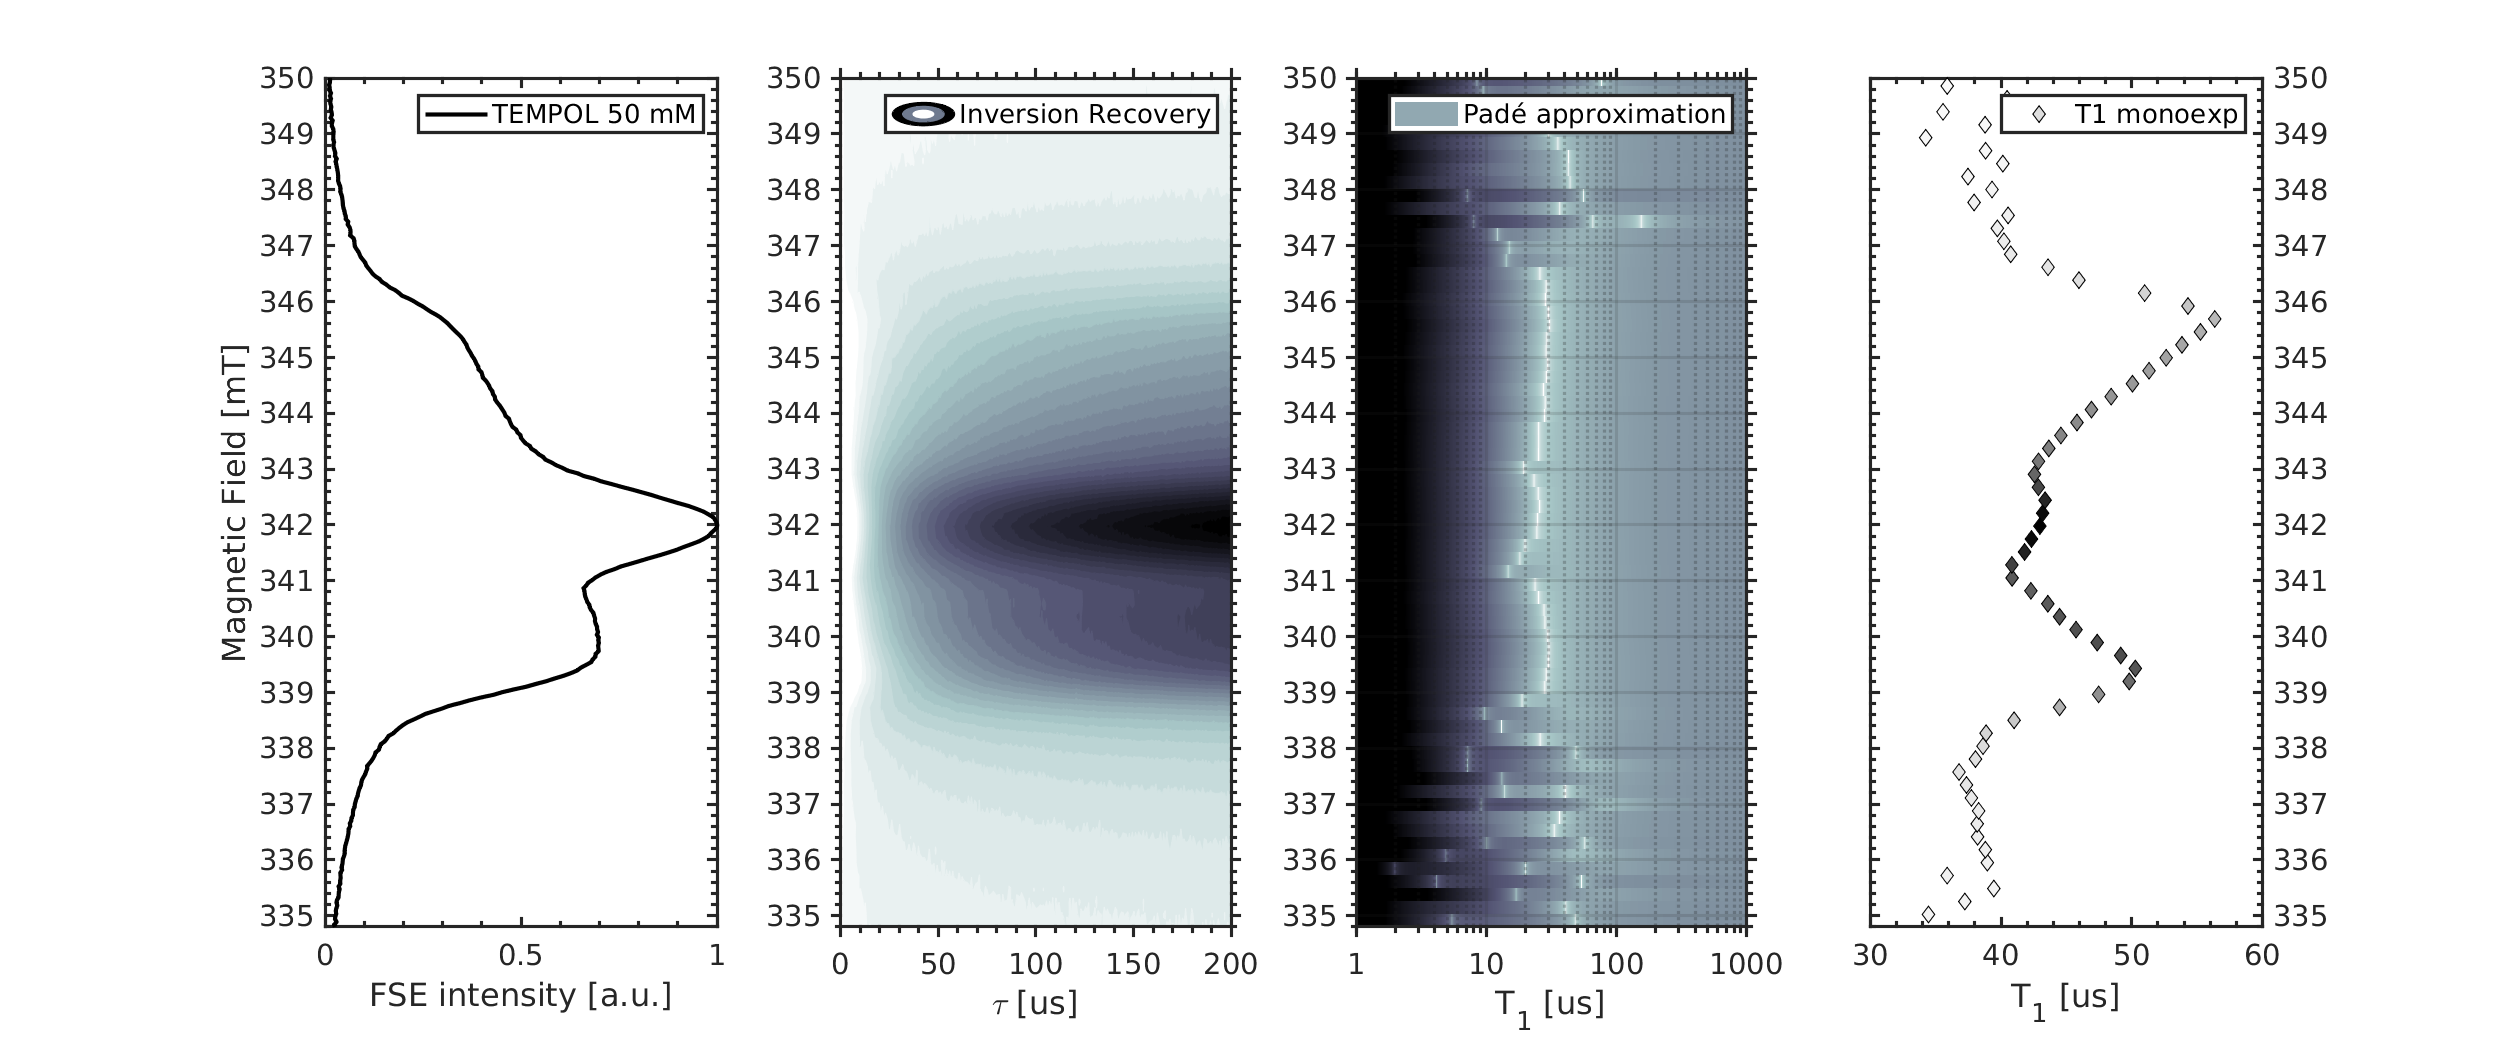
\includegraphics[width=1\textwidth]{./pulse/figures/Figure_S14.png}
	\caption{Pad{\'e}-Laplace deconvolution of the field-swept inversion recovery in a frozen 50~\si{\milli\Molar}  solution of TEMPOL in the Dichloromethane:Acetonitrile glass (3:1). Two decay components detected with Pade-Laplace (separated poles in the Pad{\'e}-Laplace approximation, third panel). Biexponential fit (circles for faster component, squares for slower component, right panel). Temperature 5K.}
	\label{fig:Figure_S14}
\end{figure}


\begin{figure}[ht!]
\center
	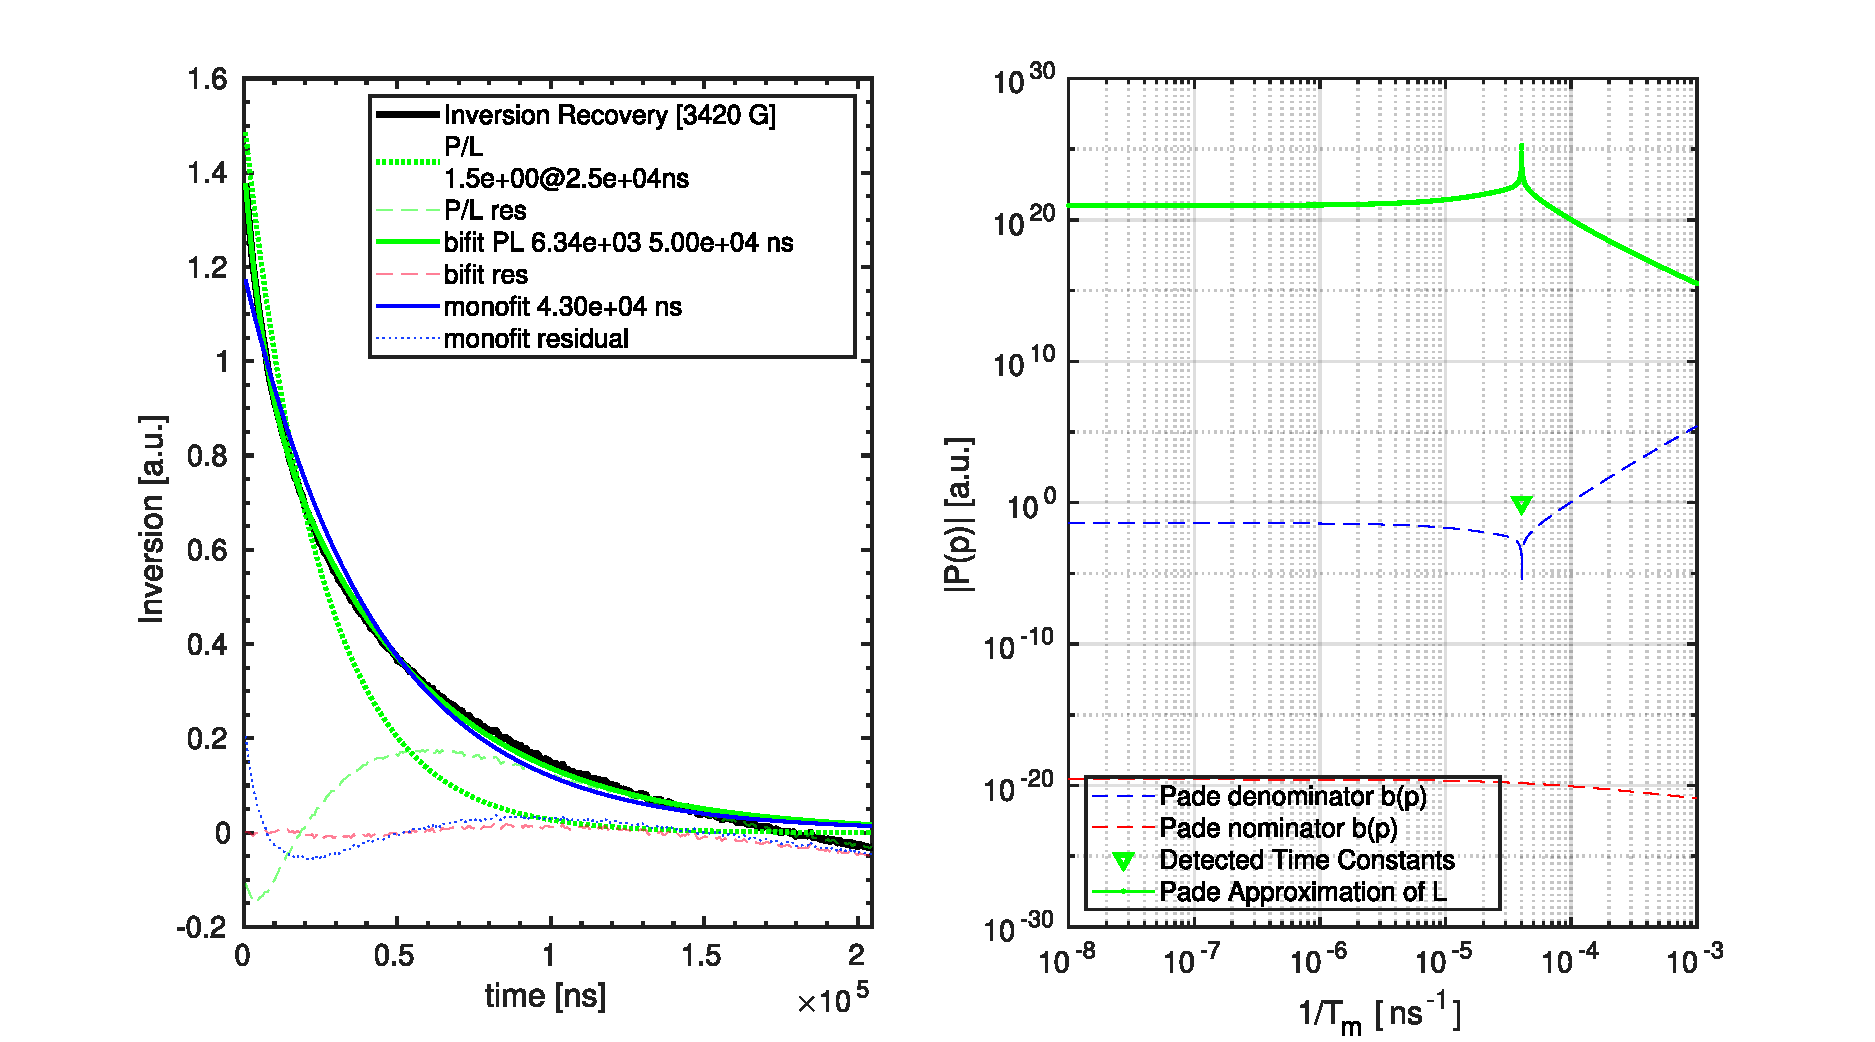
\includegraphics[width=0.9\textwidth]{./pulse/figures/Figure_S15.pdf}
	\caption{Fits of the inversion recovery transient in the frozen 50~\si{\milli\Molar}  TEMPOL solution at the central spectral peak ($m_I=0$, 342~mT). Pad{\'e}-Laplace deconvolution the transient and a biexponential fit. Temperature 5K.}
	\label{fig:Figure_S15}
\end{figure}



\newpage
\subsubsection{Inversion Recovery in DiTBuS 95\% ESOC}
\begin{figure}[h]
\center
	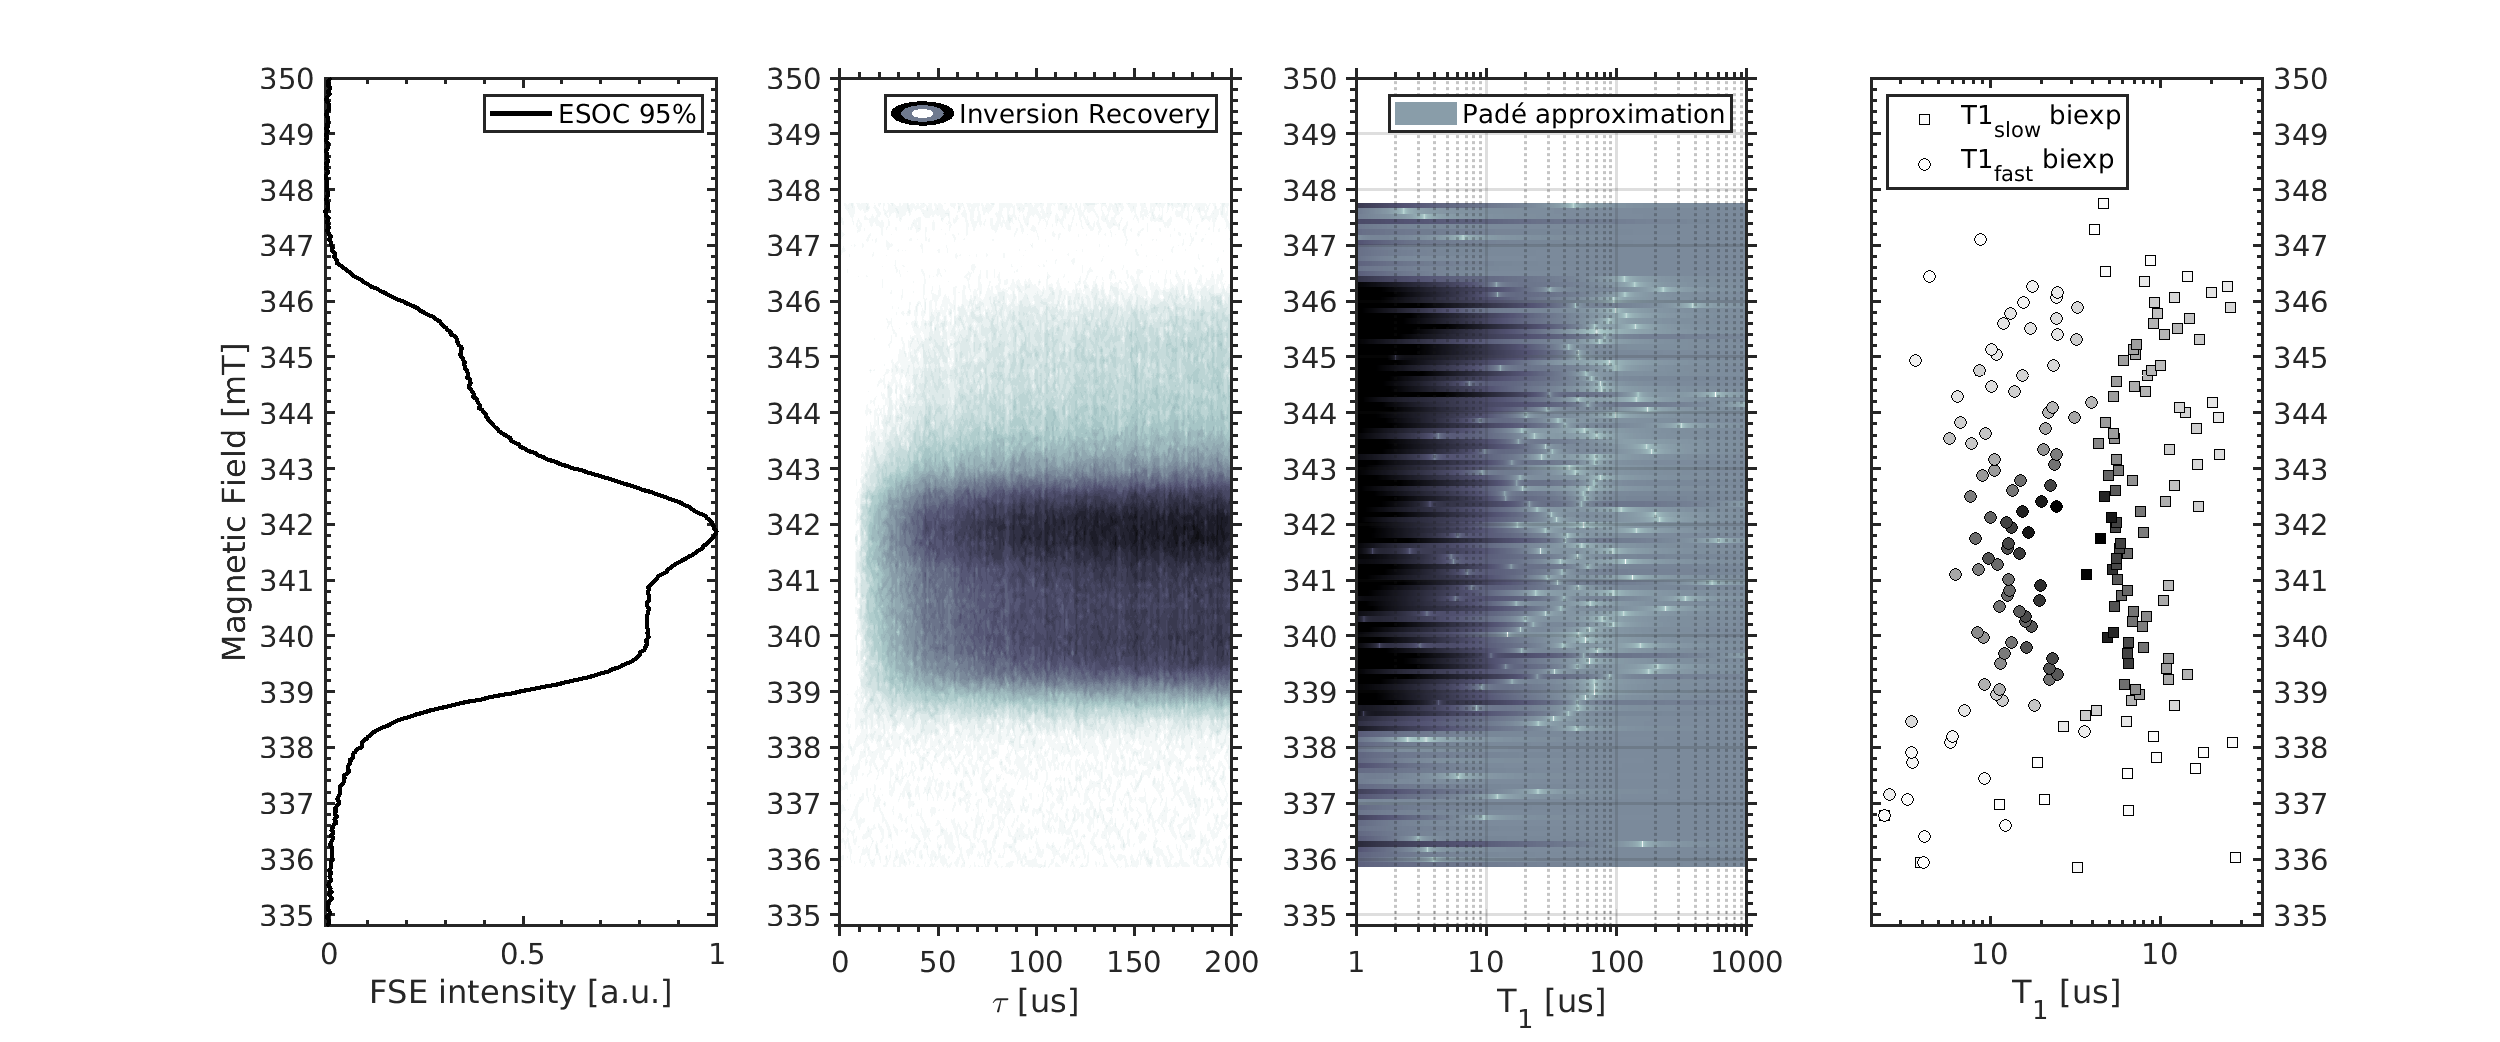
\includegraphics[width=1\textwidth]{./pulse/figures/Figure_S16.pdf}
	\caption{Pade-Laplace deconvolution of the field-swept inversion recovery in a pDiTBuS film at 95\%~ESOC. Temperature 5K.}
	\label{fig:Figure_S16}
\end{figure}

\begin{figure}[ht!]
\center
	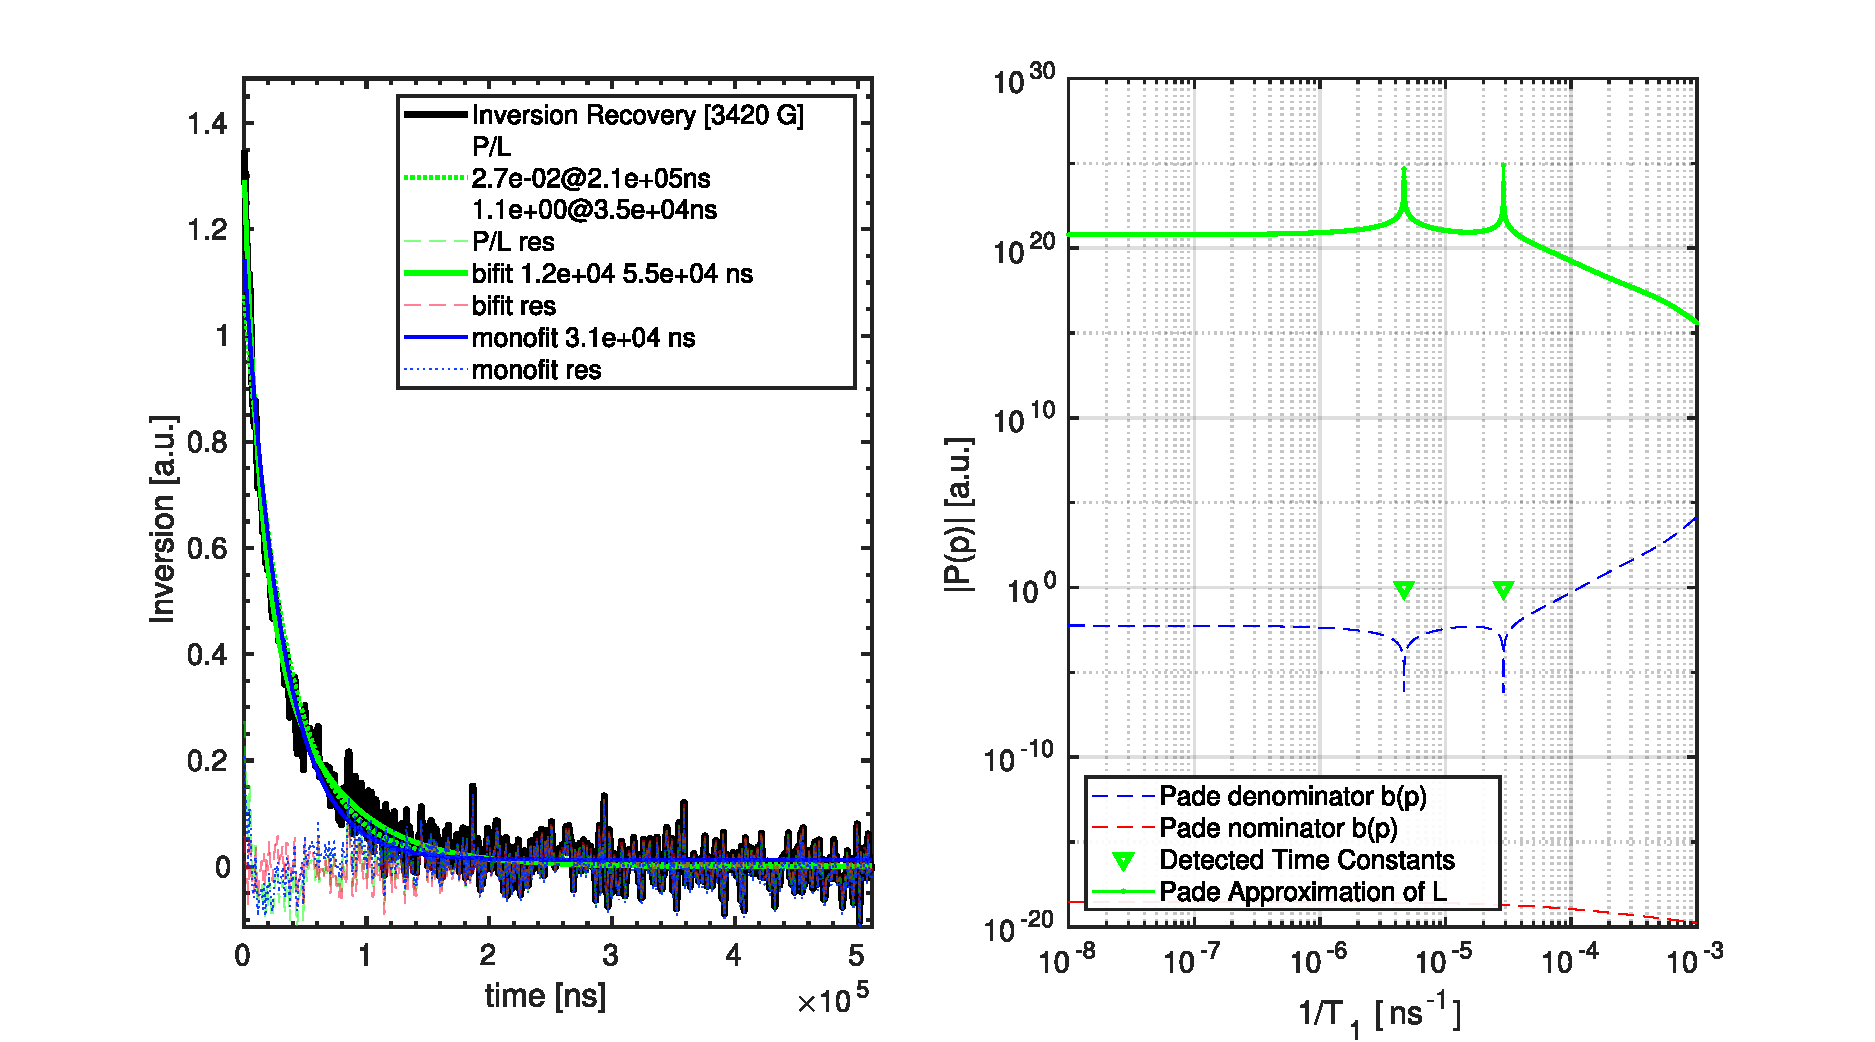
\includegraphics[width=0.9\textwidth]{./pulse/figures/Figure_S17.pdf}
	\caption{Fits of the inversion recovery transient in the 95\% ESOC pDiTBuS film at the central spectral peak ($m_I=0$, 342~mT). Pad{\'e}-Laplace deconvolution the transient and a biexponential fit. Temperature 5K.}
	\label{fig:Figure_S17}
\end{figure}


\newpage
\subsubsection{Inversion Recovery in DiTBuS 85\% ESOC}
\begin{figure}[h]
\center
	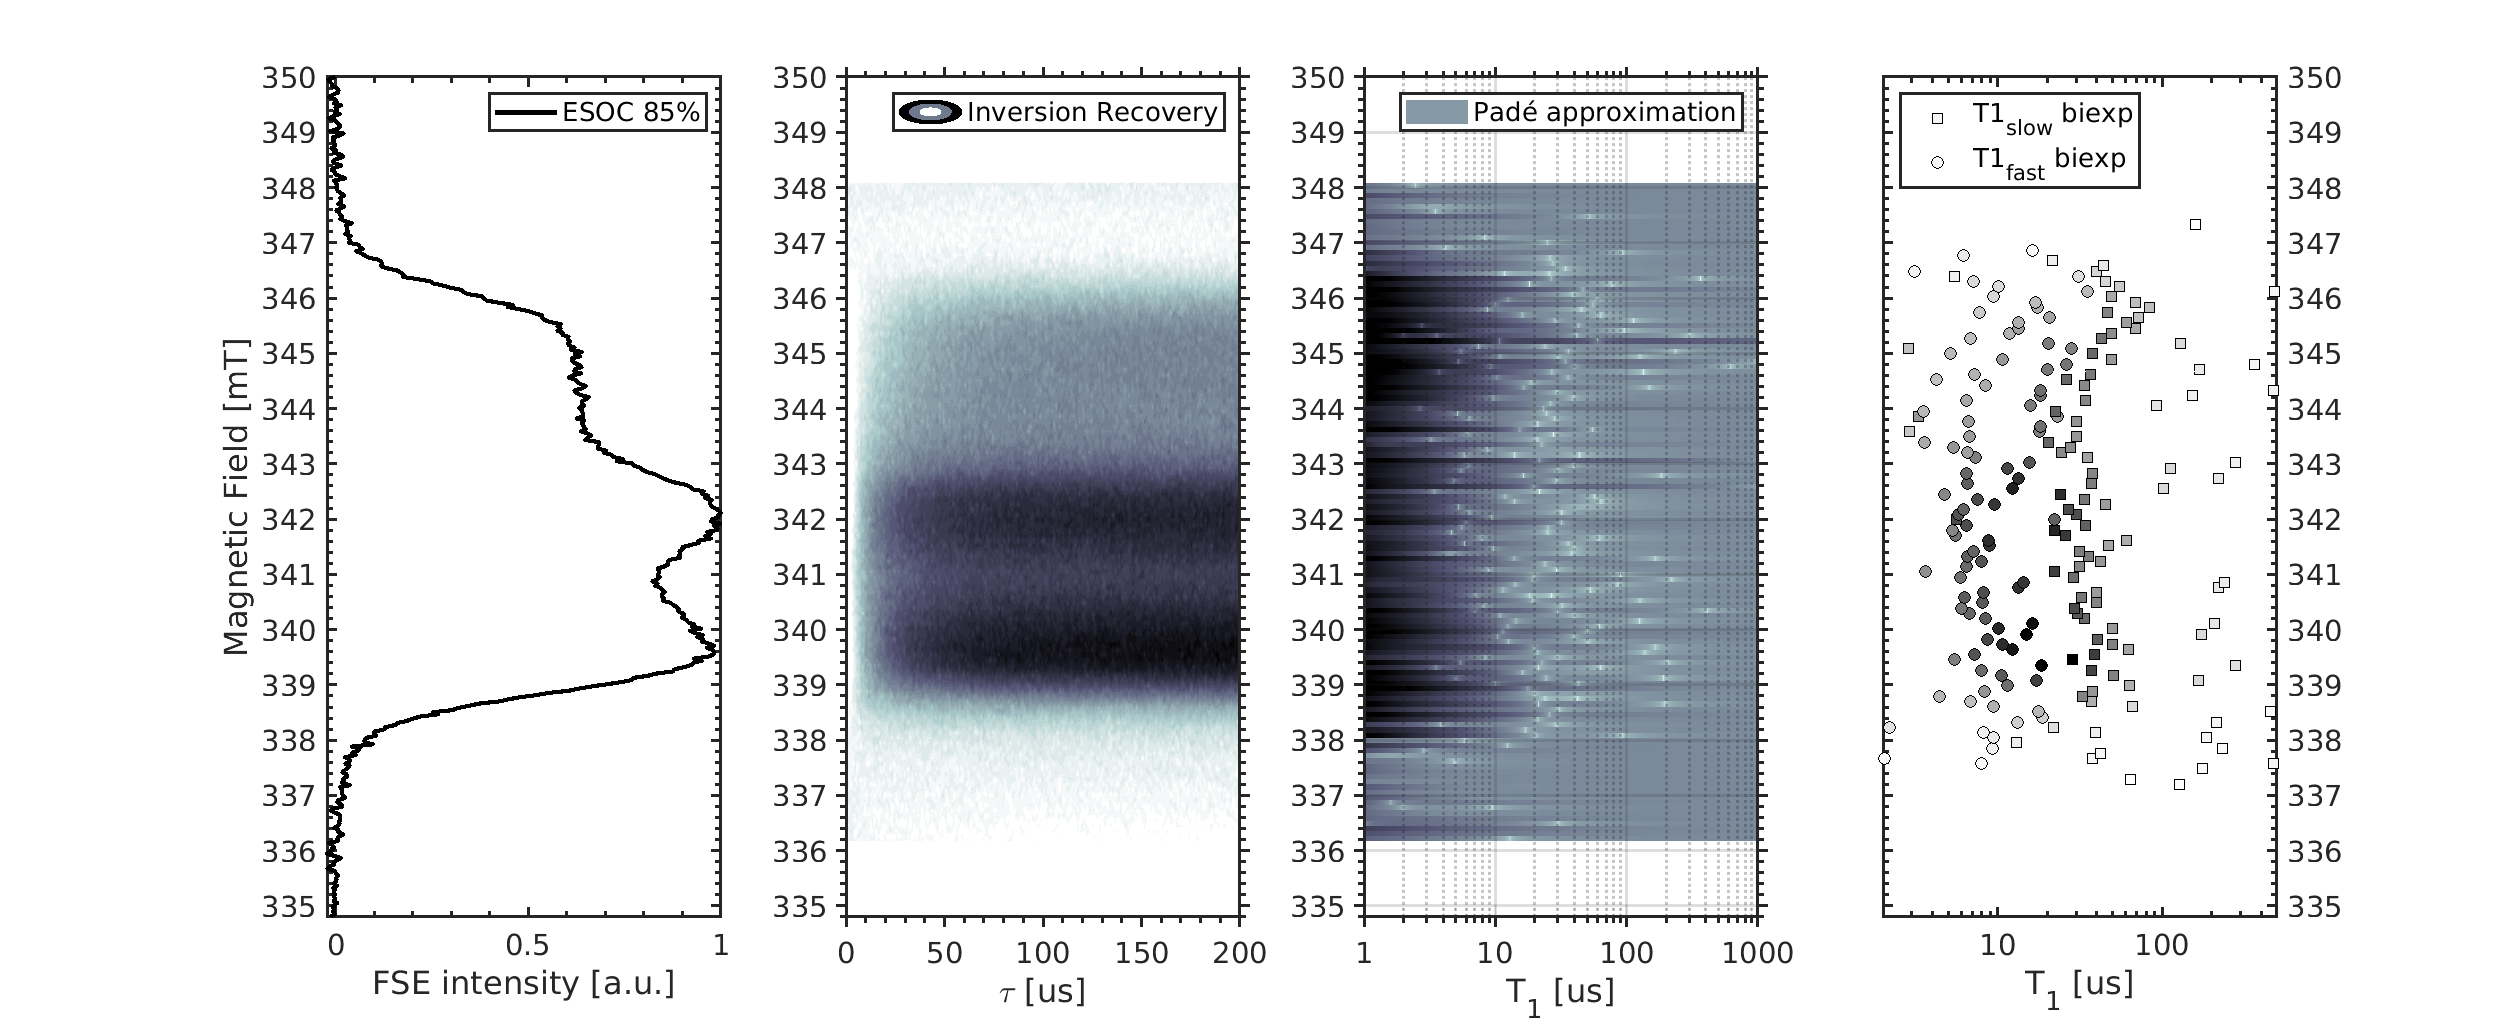
\includegraphics[width=1\textwidth]{./pulse/figures/Figure_S18.pdf}
	\caption{Pade-Laplace deconvolution of the field-swept inversion recovery in a pDiTBuS film at 85\%~ESOC. Temperature 5K.}
	\label{fig:Figure_S18}
\end{figure}


\begin{figure}[ht!]
\center
	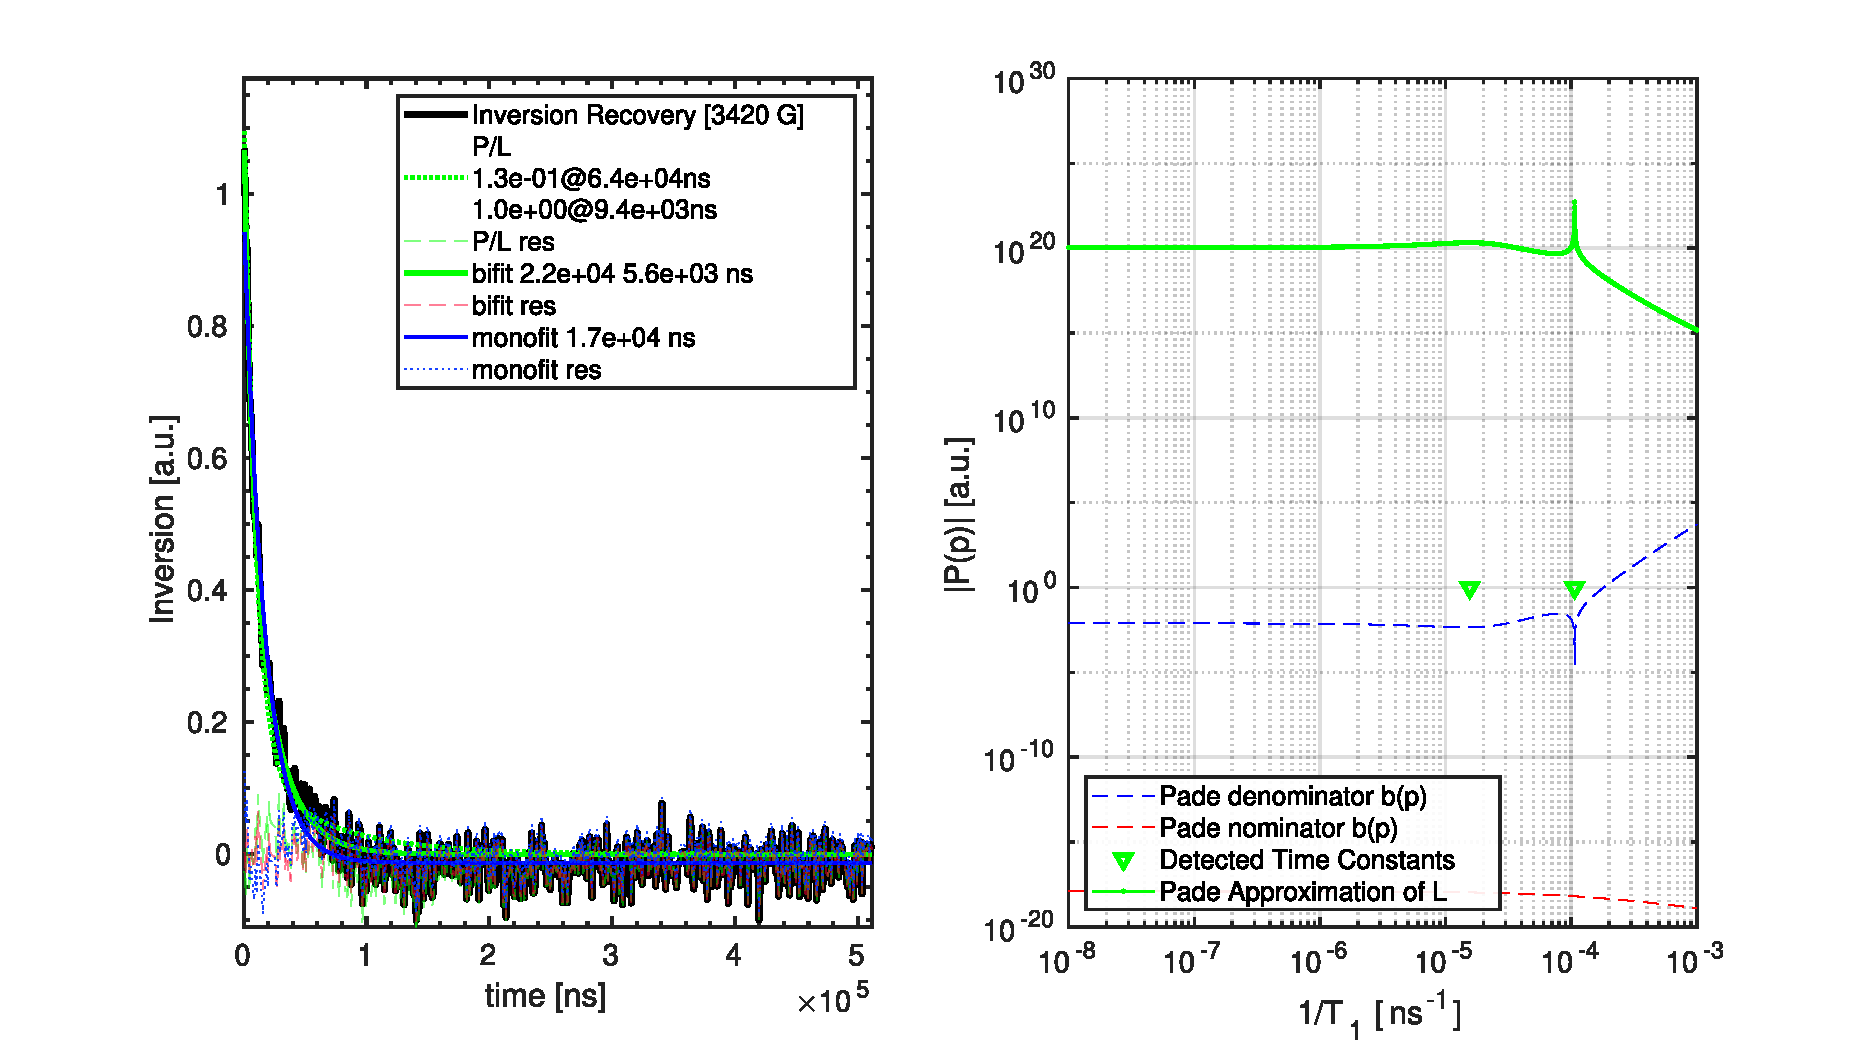
\includegraphics[width=0.9\textwidth]{./pulse/figures/Figure_S19.pdf}
	\caption{Pade-Laplace deconvolution and biexponential fit of the inversion recovery in a pDiTBuS film at 85\%~ESOC at the $m_I=0$ spectral position. Temperature 5K. Data is inverted and scaled before fitting.}
	\label{fig:Figure_S19}
\end{figure}




\subsection{\ik{Limitation on Shortest Detectable $T_m$ by the Spectrometer Dead Time}}
\label{esi:dead_time}

\ik{If a system exhibits multiple phase memory times $T_m$, the spin echo from the species with short memory times may decay below the noise level at a given pulse separation $\tau$. Figure~\ref{fig:Figure_S25} illustrates the spin echo intensity in a two-component system with $T_m^1=100$~ns and $T_m^2=25$~ns in dependence on the pulse separation $\tau$. The fast relaxing component with $T_m^2=25$~ns decays below the noise level after the dead time of $t_d=100$~ns.}

\begin{figure}[h]
\center
	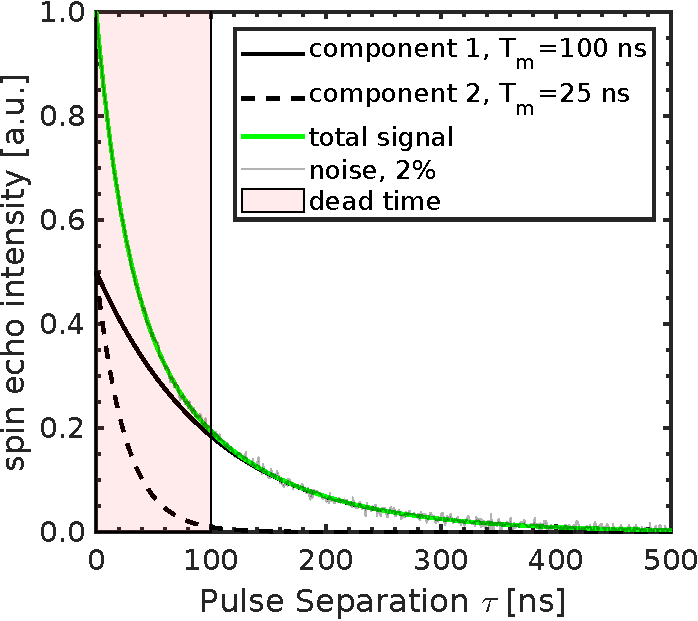
\includegraphics[width=0.6\textwidth]{./pulse/figures/Figure_S25}
	\caption{\ik{Simulated echo decay transient of a spin ensemble exhibiting two distinct phase memory times $T_m^1=100$~ns and $T_m^2=25$~ns. The 100~ns dead time, during which the spin echo detection is not possible, is marked in red. After the dead time, the sum of the two components is indistinguishable from the slowly relaxing component within the 2\% noise.}}
	\label{fig:Figure_S25}
\end{figure}




\subsection{Detection of Domains with Poor Conductivity}
\label{sec:domains_distinction_by_relaxation}

\subsection{Towards Electron Resonance Imaging of Spin Concentrations in Battery Electrodes}
The local spin concentrations that are present in an electrode film can be obtained by the time-constant-domain analysis of the echo decay transients, as it was described in \ref{sec:domains_distinction_by_relaxation}. One can extend this characterization technique and obtain a spatially resolved image of the spin concentrations inside the battery electrode by encoding the position at which the sample is excited with a gradient of the magnetic field. A strongly asymmetric ferromagnetic wedge~\cite{SternGerlach1922} can be used to superimpose a gradient of $B_0$ in a chosen direction so one can not only measure the spin concentrations that are present in the electrode, but also to locate the electrochemically inactive domains and to visualize the conductive paths throughout the electrode, analogously to the NMR imaging. The difficulty on the way to apply this visualization technique lies in the large excitation bandwidth of the pulse sequence.
\par
Let the cathode film of width $l$ be oriented along the static magnetic field so that $B_0$ lies in the film plane. Let the $B_0$ be fixed at the maximum intensity of the FSE spectrum, say, $B_0 = B_0^{res}=342$~mT. Let $B_0$ be homogeneous within the film length, which is normally the case for the EPR resonator. Let the film contain a distribution of spin concentrations within its length $C_{min}<C(z)<C_{max}$. With the homogeneous $B_0$, the microwave pulse will excite the entire film length and the spin echo signal will contain spin echoes from all length elements of the film, that correspond to all $C(z)$. The inversion recovery transient will contain the time constants from all length elements of the film $T_1(z)$. With the Pad{\'e}-Laplace analysis one recovers the distribution of the concentrations within the film $C_i$, but since the $B_0$ is homogeneous, the information on the position $z_i$ at which the domains are located, is lost. 
\par
Let now the $B_0$ to be linearly increasing from $B_0(z=-l/2) = B_0^{res}-\Delta B_0$ at one side of the film to $B_0(z=l/2)=B_0^{res}+ \Delta B_0$ by the other side of the film, so that for a given length element $dl$ the inhomogeneity of $B_0$ is $dB/dl = \frac{B(z=l/2)-B(z=-l/2)}{l}$. In the center of the film (at $z=0$) the $B_0$ is resonant and the spin echo signal will be generated, while from the other positions of the film the magnetic field will be non-resonant and no spin echo signal will be generated. Let the width of the EPR spectrum be $\Delta B_{FWHM}=8$~mT and that to define the probed length element $\Delta l$ with the given $B_0$ gradient. $\frac{\Delta B_{FWHM}}{\Delta l} = \frac{B(z=l/2)-B(z=-l/2)}{l}$, so the spatial resolution is 

\begin{equation}
\label{eq:ERI_resolution}
\frac{\Delta l}{l} = \frac{\Delta B_{FWHM}}{B(z=l/2)-B(z=-l/2)}
\end{equation}

With the spectral width of $\Delta B_{FWHM}\leq8$~mT and the film width of $l\leq3\times10^{-1}$~cm to get 
256 points per film length one needs a $B_0$ gradient of $dB/dl \geq 256*8/0.3 \geq 6.8$~[T/cm] which is a realistic value for a typical Stern-Gerlach apparatus~\cite{SternGerlach1922,Liang_2020}. 
